% Traduction française de travail du manuscrit paper/main.tex.
% Les chiffres viennent du même numbers.tex que la version anglaise.
\documentclass[11pt,a4paper]{article}

\usepackage[utf8]{inputenc}
\usepackage[T1]{fontenc}
\usepackage[margin=1in]{geometry}
\usepackage{amsmath,amssymb}
\usepackage{booktabs}
\usepackage{graphicx}
\graphicspath{{../../reports/figures/}}
\usepackage{caption}
\usepackage[hidelinks]{hyperref}
\usepackage{natbib}
\usepackage[expansion=false]{microtype}
\usepackage{setspace}
\setstretch{1.15}
\sloppy

% GENERATED by scripts/make_paper_numbers.py -- do not edit by hand.
%
% Every number in main.tex is one of these macros. The manuscript
% contains no digits of its own, so it cannot drift from the data the
% way this project's prose repeatedly has -- regenerate the artifacts,
% regenerate this file, and the paper is correct or CI fails.

\newcommand{\NDecisions}{1,280}
\newcommand{\NDecisionsFone}{357}
\newcommand{\NRaceSeasons}{205}
\newcommand{\NCircuitClasses}{51}
\newcommand{\NClasses}{7}
\newcommand{\NCircuitsFone}{25}
\newcommand{\NCoefficientsFone}{73}
\newcommand{\NRacesFoneHeldOut}{12}
\newcommand{\NRacesFone}{92}
\newcommand{\SeasonsFone}{2022--2025}
\newcommand{\NDecisionsFoneScope}{357}
\newcommand{\NRacesElms}{42}
\newcommand{\SeasonsElms}{2021--2025}
\newcommand{\NClassesElms}{2}
\newcommand{\NCircuitsElms}{9}
\newcommand{\NDecisionsElms}{171}
\newcommand{\NRacesImsa}{136}
\newcommand{\SeasonsImsa}{2021--2026}
\newcommand{\NClassesImsa}{3}
\newcommand{\NCircuitsImsa}{13}
\newcommand{\NDecisionsImsa}{632}
\newcommand{\NRacesWec}{27}
\newcommand{\SeasonsWec}{2022--2026}
\newcommand{\NClassesWec}{1}
\newcommand{\NCircuitsWec}{11}
\newcommand{\NDecisionsWec}{120}
\newcommand{\NFinishers}{5}
\newcommand{\NCars}{5}
\newcommand{\LookbackFone}{5}
\newcommand{\LookbackEnd}{3}
\newcommand{\MinFirstStopFone}{8}
\newcommand{\MinFirstStopEnd}{6}
\newcommand{\NRivals}{2}
\newcommand{\NDraws}{5,000}
\newcommand{\MinFinalStint}{3}
\newcommand{\NCoefCrossingZero}{16}
\newcommand{\PctCoefCrossingZero}{22}
\newcommand{\NFitsWec}{28}
\newcommand{\NSlopeZeroWec}{8}
\newcommand{\PctSlopeZeroWec}{29}
\newcommand{\NSlopeNegativeWec}{9}
\newcommand{\PctSlopeNegativeWec}{32}
\newcommand{\NSeparableWec}{0}
\newcommand{\MedFuelDegCorrWec}{0.992}
\newcommand{\NFitsImsa}{140}
\newcommand{\NSlopeZeroImsa}{33}
\newcommand{\PctSlopeZeroImsa}{24}
\newcommand{\NSlopeNegativeImsa}{20}
\newcommand{\PctSlopeNegativeImsa}{14}
\newcommand{\NSeparableImsa}{6}
\newcommand{\MedFuelDegCorrImsa}{0.980}
\newcommand{\NFitsElms}{42}
\newcommand{\NSlopeZeroElms}{22}
\newcommand{\PctSlopeZeroElms}{52}
\newcommand{\NSlopeNegativeElms}{12}
\newcommand{\PctSlopeNegativeElms}{29}
\newcommand{\NSeparableElms}{0}
\newcommand{\MedFuelDegCorrElms}{0.985}
\newcommand{\PctCompoundOverlap}{75}
\newcommand{\BestTransfer}{+0.573}
\newcommand{\BestTransferWhere}{Lime Rock GTD}
\newcommand{\TransferThreshold}{0.2}
\newcommand{\NTransferAboveTwo}{5}
\newcommand{\GTThreeMean}{+0.104}
\newcommand{\GTThreeCI}{[+0.050, +0.170]}
\newcommand{\ProtoMean}{-0.060}
\newcommand{\ProtoCI}{[-0.199, +0.021]}
\newcommand{\TransferDiff}{+0.164}
\newcommand{\TransferDiffCI}{[+0.059, +0.312]}
\newcommand{\TransferP}{0.0011}
\newcommand{\NReportedTests}{5}
\newcommand{\NClassPartitions}{31}
\newcommand{\TransferPBonferroni}{0.034}
\newcommand{\BonferroniBreakeven}{46}
\newcommand{\RegimeAucPitLoss}{0.977}
\newcommand{\RegimeAucPitLossCI}{[0.955, 0.994]}
\newcommand{\RegimeAucSlope}{0.865}
\newcommand{\RegimeAucSlopeCI}{[0.806, 0.915]}
\newcommand{\RegimeNTyreLimited}{25}
\newcommand{\RegimeNFuelLimited}{180}
\newcommand{\DOneDecisions}{357}
\newcommand{\DOneNoRival}{91}
\newcommand{\DOneChasers}{266}
\newcommand{\DOnePredicted}{254}
\newcommand{\DOneMedianGap}{3.4}
\newcommand{\DOneWithinPitLoss}{260}
\newcommand{\DOneReachable}{266}
\newcommand{\DOneMedianError}{+55}
\newcommand{\DOneBaselineError}{+9}
\newcommand{\DOneCloser}{41}
\newcommand{\DOneFurther}{207}
\newcommand{\DOneImpliedTheta}{0.185}
\newcommand{\DOneMeasuredTheta}{0.045}
\newcommand{\DOneThetaRatio}{3.4}
\newcommand{\DOneThetaRatioIQR}{1.4 to 8.6}
\newcommand{\DOnePctThetaAbove}{79}
\newcommand{\DOneThetaPercentile}{99}
\newcommand{\DOneMaxGap}{36}
\newcommand{\DOnePctAgeIsLap}{78}
\newcommand{\DOneStaleDropped}{85}
\newcommand{\NRivalRules}{4}
\newcommand{\RivalPositionScored}{357}
\newcommand{\RivalPositionAdv}{+11}
\newcommand{\RivalPositionClosed}{-1}
\newcommand{\RivalPositionMeanClosed}{-0.96}
\newcommand{\RivalPositionBetter}{63}
\newcommand{\RivalPositionWorse}{200}
\newcommand{\RivalThravesScored}{357}
\newcommand{\RivalThravesAdv}{+10}
\newcommand{\RivalThravesClosed}{+0}
\newcommand{\RivalThravesMeanClosed}{-0.01}
\newcommand{\RivalThravesBetter}{99}
\newcommand{\RivalThravesWorse}{176}
\newcommand{\RivalPiWindowScored}{357}
\newcommand{\RivalPiWindowAdv}{+11}
\newcommand{\RivalPiWindowClosed}{-1}
\newcommand{\RivalPiWindowMeanClosed}{-1.06}
\newcommand{\RivalPiWindowBetter}{55}
\newcommand{\RivalPiWindowWorse}{213}
\newcommand{\RivalDOneScored}{271}
\newcommand{\RivalDOneAdv}{+11}
\newcommand{\RivalDOneClosed}{-1}
\newcommand{\RivalDOneMeanClosed}{-0.75}
\newcommand{\RivalDOneBetter}{56}
\newcommand{\RivalDOneWorse}{147}
\newcommand{\NRivalAllApply}{271}
\newcommand{\NRivalAllAgree}{17}
\newcommand{\NRivalTwoCars}{148}
\newcommand{\NRivalThreeCars}{106}
\newcommand{\MaxRivalCars}{3}
\newcommand{\RivalPairMin}{20}
\newcommand{\RivalPairMax}{65}
\newcommand{\RivalPairMedian}{36}
\newcommand{\PctRivalThravesAgrees}{20}
\newcommand{\RivalStandaloneGap}{4.0}
\newcommand{\NTiedDecisions}{271}
\newcommand{\NCatalogued}{17}
\newcommand{\NBlockedLayers}{3}
\newcommand{\BestTransferFolds}{3}
\newcommand{\BestTransferSpread}{0.024}
\newcommand{\ThinTransfer}{+0.497}
\newcommand{\ThinTransferWhere}{Lime Rock GTD PRO}
\newcommand{\ThinTransferFolds}{2}
\newcommand{\ThinTransferLow}{+0.357}
\newcommand{\ThinTransferHigh}{+0.638}
\newcommand{\ThinTransferSpread}{0.281}
\newcommand{\PitLossR}{-0.982}
\newcommand{\PitLossRCI}{[-0.986, -0.745]}
\newcommand{\CheapStopEdge}{22.5}
\newcommand{\NAboveEdge}{150}
\newcommand{\NTyreLimitedAboveEdge}{0}
\newcommand{\NTyreLimited}{25}
\newcommand{\EdgeWithoutDefining}{13.2}
\newcommand{\EdgeDropPct}{41}
\newcommand{\FoneMedian}{+10}
\newcommand{\FoneLateShare}{80}
\newcommand{\FoneLateMedian}{12}
\newcommand{\ElmsMedian}{+2}
\newcommand{\ElmsLateShare}{56}
\newcommand{\ElmsCautionShare}{20}
\newcommand{\ImsaMedian}{+12}
\newcommand{\ImsaLateShare}{83}
\newcommand{\ImsaCautionShare}{53}
\newcommand{\WecMedian}{+1}
\newcommand{\WecLateShare}{30}
\newcommand{\WecCautionShare}{8}
\newcommand{\NScored}{1,263}
\newcommand{\ElmsLmptwoModelError}{2}
\newcommand{\ElmsLmptwoBoneError}{3}
\newcommand{\ElmsLmptwoBtwoError}{45}
\newcommand{\ElmsLmptwoBthreeError}{4}
\newcommand{\ElmsLmptwoCommitError}{2}
\newcommand{\ElmsLmptwoProAmModelError}{3}
\newcommand{\ElmsLmptwoProAmBoneError}{2}
\newcommand{\ElmsLmptwoProAmBtwoError}{45}
\newcommand{\ElmsLmptwoProAmBthreeError}{4}
\newcommand{\ElmsLmptwoProAmCommitError}{2}
\newcommand{\FoneModelError}{10}
\newcommand{\FoneBoneError}{11}
\newcommand{\FoneBtwoError}{7}
\newcommand{\FoneBthreeError}{--}
\newcommand{\FoneCommitError}{4}
\newcommand{\ImsaGtdModelError}{12}
\newcommand{\ImsaGtdBoneError}{7}
\newcommand{\ImsaGtdBtwoError}{18}
\newcommand{\ImsaGtdBthreeError}{14}
\newcommand{\ImsaGtdCommitError}{2}
\newcommand{\ImsaGtdproModelError}{12}
\newcommand{\ImsaGtdproBoneError}{9}
\newcommand{\ImsaGtdproBtwoError}{33}
\newcommand{\ImsaGtdproBthreeError}{15}
\newcommand{\ImsaGtdproCommitError}{2}
\newcommand{\ImsaGtpModelError}{9}
\newcommand{\ImsaGtpBoneError}{9}
\newcommand{\ImsaGtpBtwoError}{54}
\newcommand{\ImsaGtpBthreeError}{14}
\newcommand{\ImsaGtpCommitError}{2}
\newcommand{\WecHypercarModelError}{2}
\newcommand{\WecHypercarBoneError}{2}
\newcommand{\WecHypercarBtwoError}{39}
\newcommand{\WecHypercarBthreeError}{1}
\newcommand{\WecHypercarCommitError}{1}
\newcommand{\NClassesRuleWins}{5}
\newcommand{\NClassesBoneWins}{3}
\newcommand{\NClassesRuleTies}{1}
\newcommand{\NClassesOptimiserWins}{1}
\newcommand{\NClassesScored}{7}
\newcommand{\NClassesCommitBeatsRules}{5}
\newcommand{\NClassesCommitTiesRules}{2}
\newcommand{\NClassesCommitLosesRules}{0}
\newcommand{\PrecisionHalfSlopeAuc}{0.872}
\newcommand{\PrecisionHalfPitAuc}{0.964}
\newcommand{\NPrecisionHalf}{103}
\newcommand{\PrecisionThirdSlopeAuc}{0.815}
\newcommand{\PrecisionThirdPitAuc}{0.964}
\newcommand{\NPrecisionThird}{68}
\newcommand{\NPrecisionThirdTyreLimited}{8}
\newcommand{\ElmsLmptwoPitLoss}{62}
\newcommand{\ElmsLmptwoProAmPitLoss}{64}
\newcommand{\ImsaGtdPitLoss}{24}
\newcommand{\ImsaGtdproPitLoss}{40}
\newcommand{\ImsaGtpPitLoss}{57}
\newcommand{\WecHypercarPitLoss}{74}
\newcommand{\TrackPositionRange}{14}
\newcommand{\NCircuitsSwap}{25}
\newcommand{\SwapLowestCircuit}{Monaco}
\newcommand{\SwapHighestCircuit}{Las Vegas}
\newcommand{\SwapLowest}{0.0047}
\newcommand{\SwapLowestSd}{0.0016}
\newcommand{\SwapLowestRaces}{4}
\newcommand{\SwapHighestRaces}{3}
\newcommand{\SwapRunnerUpRatio}{4.1}
\newcommand{\SwapBetweenSd}{0.0104}
\newcommand{\SwapWithinSd}{0.0103}
\newcommand{\UndercutClosedMedian}{-1}
\newcommand{\UndercutShareImproving}{18}
\newcommand{\UndercutSpearman}{-0.16}
\newcommand{\SwapLowestClosedMedian}{+0.5}
\newcommand{\SwapLowestDecisions}{8}
\newcommand{\NIdentifiability}{0.691}
\newcommand{\AuditCiFone}{[+8, +11.5]}
\newcommand{\AuditCiLowFone}{+8.0}
\newcommand{\AuditCiHighFone}{+11.5}
\newcommand{\AuditMedFone}{+10}
\newcommand{\AuditRacesFone}{74}
\newcommand{\AuditCiImsaGtd}{[+8, +14]}
\newcommand{\AuditCiLowImsaGtd}{+8.0}
\newcommand{\AuditCiHighImsaGtd}{+14.0}
\newcommand{\AuditMedImsaGtd}{+12}
\newcommand{\AuditRacesImsaGtd}{58}
\newcommand{\AuditCiImsaGtdpro}{[+9, +16]}
\newcommand{\AuditCiLowImsaGtdpro}{+9.0}
\newcommand{\AuditCiHighImsaGtdpro}{+16.0}
\newcommand{\AuditMedImsaGtdpro}{+13}
\newcommand{\AuditRacesImsaGtdpro}{46}
\newcommand{\AuditCiImsaGtp}{[+5, +15]}
\newcommand{\AuditCiLowImsaGtp}{+5.0}
\newcommand{\AuditCiHighImsaGtp}{+15.0}
\newcommand{\AuditMedImsaGtp}{+9}
\newcommand{\AuditRacesImsaGtp}{32}
\newcommand{\AuditCiWecHypercar}{[0, +1]}
\newcommand{\AuditCiLowWecHypercar}{+0.0}
\newcommand{\AuditCiHighWecHypercar}{+1.0}
\newcommand{\AuditMedWecHypercar}{+1}
\newcommand{\AuditRacesWecHypercar}{26}
\newcommand{\AuditCiElmsLmptwo}{[-1, +3]}
\newcommand{\AuditCiLowElmsLmptwo}{-1.0}
\newcommand{\AuditCiHighElmsLmptwo}{+3.0}
\newcommand{\AuditMedElmsLmptwo}{+2}
\newcommand{\AuditRacesElmsLmptwo}{24}
\newcommand{\AuditCiElmsLmptwoProAm}{[+1, +4]}
\newcommand{\AuditCiLowElmsLmptwoProAm}{+1.0}
\newcommand{\AuditCiHighElmsLmptwoProAm}{+4.0}
\newcommand{\AuditMedElmsLmptwoProAm}{+3}
\newcommand{\AuditRacesElmsLmptwoProAm}{15}
\newcommand{\AuditCiEndurance}{[+4, +9]}
\newcommand{\AuditCiLowEndurance}{+4.0}
\newcommand{\AuditCiHighEndurance}{+9.0}
\newcommand{\AuditMedEndurance}{+7}
\newcommand{\AuditRacesEndurance}{111}
\newcommand{\NAuditContainsZero}{2}
\newcommand{\AuditZeroClasses}{HYPERCAR, LMP2}
\newcommand{\NAuditScopes}{7}
\newcommand{\NCeilingCircuits}{22}
\newcommand{\NCeilingBelowThreshold}{16}
\newcommand{\NCeilingUnstable}{11}
\newcommand{\NCeilingStable}{1}
\newcommand{\NCeilingNoSignal}{7}
\newcommand{\NCeilingBorderline}{3}
\newcommand{\CeilingLowest}{+0.011}
\newcommand{\CeilingLowestWhere}{Zandvoort}
\newcommand{\CeilingHighest}{+0.439}
\newcommand{\CeilingHighestWhere}{Jeddah}
\newcommand{\LeakageMean}{0.0178}
\newcommand{\LeakageMax}{0.2290}
\newcommand{\NCeilingExcluded}{1}
\newcommand{\FreshAge}{2}
\newcommand{\FreshResid}{+0.187}
\newcommand{\FreshResidNext}{+0.059}
\newcommand{\FreshAgeNext}{3}
\newcommand{\NFreshCircuits}{24}
\newcommand{\NFreshFaster}{7}
\newcommand{\FreshMedianBonus}{-0.048}
\newcommand{\CommitAllBefore}{+9.5}
\newcommand{\CommitAllAfter}{+2}
\newcommand{\CommitAllCi}{[+1, +4]}
\newcommand{\CommitAllCiLow}{+1.0}
\newcommand{\CommitAllCiHigh}{+4.0}
\newcommand{\CommitAllBeforeCi}{[+8, +11]}
\newcommand{\NCommitAll}{352}
\newcommand{\CommitOneBefore}{+4}
\newcommand{\CommitOneAfter}{+4}
\newcommand{\CommitOneCi}{[+2, +7]}
\newcommand{\CommitOneCiLow}{+2.0}
\newcommand{\CommitOneCiHigh}{+7.0}
\newcommand{\CommitOneBeforeCi}{[+2, +7]}
\newcommand{\NCommitOne}{150}
\newcommand{\CommitMultiBefore}{+12}
\newcommand{\CommitMultiAfter}{+1}
\newcommand{\CommitMultiCi}{[+1, +2]}
\newcommand{\CommitMultiCiLow}{+1.0}
\newcommand{\CommitMultiCiHigh}{+2.0}
\newcommand{\CommitMultiBeforeCi}{[+11, +14]}
\newcommand{\NCommitMulti}{202}
\newcommand{\CommitThreeBefore}{+17}
\newcommand{\CommitThreeAfter}{+2}
\newcommand{\CommitThreeCi}{[-1, +4]}
\newcommand{\CommitThreeCiLow}{-1.0}
\newcommand{\CommitThreeCiHigh}{+4.0}
\newcommand{\CommitThreeBeforeCi}{[+12, +25]}
\newcommand{\NCommitThree}{43}
\newcommand{\CommitGreenBefore}{+12}
\newcommand{\CommitGreenAfter}{+2}
\newcommand{\CommitGreenCi}{[+1, +2]}
\newcommand{\CommitGreenCiLow}{+1.0}
\newcommand{\CommitGreenCiHigh}{+2.0}
\newcommand{\CommitGreenBeforeCi}{[+11, +14]}
\newcommand{\NCommitGreen}{155}
\newcommand{\CommitWindow}{24}
\newcommand{\CommitEngineMiss}{3}
\newcommand{\CommitUniformMiss}{8.3}
\newcommand{\CommitMidpointMiss}{7.5}
\newcommand{\NCommitDropped}{5}
\newcommand{\NCommitWithinRaces}{19}
\newcommand{\CommitWithinGap}{+5}
\newcommand{\EndCommitElmsLmptwoBefore}{+1}
\newcommand{\EndCommitElmsLmptwoAfter}{0}
\newcommand{\EndCommitElmsLmptwoCi}{[-1, +1]}
\newcommand{\EndCommitElmsLmptwoWindow}{6}
\newcommand{\EndCommitElmsLmptwoMiss}{2}
\newcommand{\EndCommitElmsLmptwoUniform}{1.5}
\newcommand{\EndCommitElmsLmptwoMidpoint}{1.0}
\newcommand{\EndCommitElmsLmptwoProAmBefore}{+3}
\newcommand{\EndCommitElmsLmptwoProAmAfter}{-1}
\newcommand{\EndCommitElmsLmptwoProAmCi}{[-1.5, +0.5]}
\newcommand{\EndCommitElmsLmptwoProAmWindow}{7}
\newcommand{\EndCommitElmsLmptwoProAmMiss}{2}
\newcommand{\EndCommitElmsLmptwoProAmUniform}{1.9}
\newcommand{\EndCommitElmsLmptwoProAmMidpoint}{1.0}
\newcommand{\EndCommitImsaGtdBefore}{+11}
\newcommand{\EndCommitImsaGtdAfter}{+1}
\newcommand{\EndCommitImsaGtdCi}{[0, +2]}
\newcommand{\EndCommitImsaGtdWindow}{12}
\newcommand{\EndCommitImsaGtdMiss}{2}
\newcommand{\EndCommitImsaGtdUniform}{4.5}
\newcommand{\EndCommitImsaGtdMidpoint}{4.0}
\newcommand{\EndCommitImsaGtdproBefore}{+13}
\newcommand{\EndCommitImsaGtdproAfter}{+1}
\newcommand{\EndCommitImsaGtdproCi}{[0, +5]}
\newcommand{\EndCommitImsaGtdproWindow}{13}
\newcommand{\EndCommitImsaGtdproMiss}{2}
\newcommand{\EndCommitImsaGtdproUniform}{5.0}
\newcommand{\EndCommitImsaGtdproMidpoint}{4.8}
\newcommand{\EndCommitImsaGtpBefore}{+8}
\newcommand{\EndCommitImsaGtpAfter}{0}
\newcommand{\EndCommitImsaGtpCi}{[-2, +2]}
\newcommand{\EndCommitImsaGtpWindow}{10}
\newcommand{\EndCommitImsaGtpMiss}{2}
\newcommand{\EndCommitImsaGtpUniform}{2.9}
\newcommand{\EndCommitImsaGtpMidpoint}{2.2}
\newcommand{\EndCommitWecHypercarBefore}{+1}
\newcommand{\EndCommitWecHypercarAfter}{0}
\newcommand{\EndCommitWecHypercarCi}{[-1, 0]}
\newcommand{\EndCommitWecHypercarWindow}{4}
\newcommand{\EndCommitWecHypercarMiss}{1}
\newcommand{\EndCommitWecHypercarUniform}{1.0}
\newcommand{\EndCommitWecHypercarMidpoint}{0.5}
\newcommand{\NEndCommit}{784}
\newcommand{\NEndCommitClasses}{6}
\newcommand{\NEndCommitContainsZero}{6}
\newcommand{\NEndCommitInformative}{3}
\newcommand{\RegimeAucStandardised}{0.977}
\newcommand{\RegimeAucClassLabel}{0.760}
\newcommand{\RegimeWithinClassShare}{92}
\newcommand{\NRegimeWithinClass}{4}
\newcommand{\NRegimeClassesOneRegime}{2}
\newcommand{\RegimeWithinClassMin}{0.963}
\newcommand{\RegimeWithinClassMax}{1.000}
\newcommand{\NAllocationRaces}{92}
\newcommand{\NAllocationPirelli}{50}
\newcommand{\NCompoundCircuits}{23}
\newcommand{\NCompoundChanged}{15}
\newcommand{\CompoundRelative}{0.005}
\newcommand{\CompoundReal}{-0.012}
\newcommand{\CompoundDiff}{-0.012}
\newcommand{\CompoundDiffCi}{[-0.349, +0.001]}
\newcommand{\NCompoundBetter}{4}
\newcommand{\NCompoundWorse}{11}
\newcommand{\CompoundSignP}{0.12}
\newcommand{\CompoundMaxGain}{+0.017}
\newcommand{\CompoundLinearDiff}{-0.004}
\newcommand{\CompoundLinearDiffCi}{[-0.023, +0.001]}
\newcommand{\NCompoundLinearBetter}{5}
\newcommand{\NCompoundLinearWorse}{10}
\newcommand{\NCompoundMoved}{16}
\newcommand{\NCompoundDegenerate}{1}
\newcommand{\NCompoundUnstable}{9}
\newcommand{\NCompoundUnstableBetter}{3}
\newcommand{\NCompoundUnstableWorse}{6}
\newcommand{\CompoundUnstableMin}{-0.357}
\newcommand{\CompoundUnstableMax}{+0.017}
\newcommand{\CompoundUnstableMedian}{-0.019}
\newcommand{\CompoundUnseenPct}{2.9}
\newcommand{\CompoundUnseenMaxPct}{10.7}
\newcommand{\NFridayRaces}{56}
\newcommand{\NFridayCircuits}{24}
\newcommand{\NFridaySprint}{14}
\newcommand{\FridayOther}{0.021}
\newcommand{\FridayRaw}{-0.502}
\newcommand{\FridayCorrected}{-0.339}
\newcommand{\FridayBoth}{-0.054}
\newcommand{\FridayOffset}{+0.059}
\newcommand{\FridayRawDiff}{-0.541}
\newcommand{\FridayRawDiffCi}{[-1.127, -0.236]}
\newcommand{\NFridayRawBetter}{12}
\newcommand{\NFridayRawWorse}{44}
\newcommand{\FridayCorrectedDiff}{-0.400}
\newcommand{\FridayCorrectedDiffCi}{[-0.691, -0.124]}
\newcommand{\NFridayCorrectedBetter}{11}
\newcommand{\NFridayCorrectedWorse}{45}
\newcommand{\FridayBothDiff}{-0.051}
\newcommand{\FridayBothDiffCi}{[-0.119, -0.022]}
\newcommand{\NFridayBothBetter}{17}
\newcommand{\NFridayBothWorse}{39}
\newcommand{\NFridayOtherAbove}{13}
\newcommand{\NFridayRawAbove}{6}
\newcommand{\NFridayBothAbove}{9}
\newcommand{\NRetest}{150}
\newcommand{\NRetestRules}{4}
\newcommand{\RetestCloser}{34}
\newcommand{\RetestFurther}{74}
\newcommand{\RetestCloserMax}{37}
\newcommand{\RetestFurtherMin}{55}
\newcommand{\RetestSignPMax}{0.006}
\newcommand{\NRetestLeaders}{39}
\newcommand{\NRetestPredicted}{109}
\newcommand{\RetestEuuError}{+73}
\newcommand{\RetestSingleError}{+5}
\newcommand{\RetestEuuCloser}{9}
\newcommand{\RetestEuuFurther}{97}
\newcommand{\NRetestEuuAfterFlag}{72}
\newcommand{\NRetestEuuInside}{37}
\newcommand{\RetestEuuInsideAbsDiff}{+9}
\newcommand{\RetestEuuInsideAbsDiffCi}{[+1, +15]}
\newcommand{\RetestEuuInsideCloser}{9}
\newcommand{\RetestEuuInsideFurther}{25}
\newcommand{\DesignAllTenN}{962}
\newcommand{\DesignAllTenMedian}{+2}
\newcommand{\DesignAllTenCi}{[+1, +3]}
\newcommand{\DesignAllTenHl}{+2}
\newcommand{\DesignAllTenOneMedian}{+3}
\newcommand{\DesignAllTenOneCi}{[+1, +4]}
\newcommand{\DesignAllTenOneHl}{+2.5}
\newcommand{\DesignAllTenBound}{10}
\newcommand{\DesignAllFifteenN}{670}
\newcommand{\DesignAllFifteenMedian}{+1}
\newcommand{\DesignAllFifteenCi}{[0, +2]}
\newcommand{\DesignAllFifteenHl}{+0.5}
\newcommand{\DesignAllFifteenOneMedian}{+1}
\newcommand{\DesignAllFifteenOneCi}{[-1, +3]}
\newcommand{\DesignAllFifteenOneHl}{+0.5}
\newcommand{\DesignAllFifteenBound}{10}
\newcommand{\DesignAllFiveN}{1,152}
\newcommand{\DesignAllFiveMedian}{+3}
\newcommand{\DesignAllFiveCi}{[+2, +3]}
\newcommand{\DesignAllFiveHl}{+3}
\newcommand{\DesignAllFiveOneMedian}{+4}
\newcommand{\DesignAllFiveOneCi}{[+2, +5]}
\newcommand{\DesignAllFiveOneHl}{+4.5}
\newcommand{\DesignAllFiveBound}{15}
\newcommand{\DesignTopTenN}{320}
\newcommand{\DesignTopTenMedian}{+2}
\newcommand{\DesignTopTenCi}{[+1, +4]}
\newcommand{\DesignTopTenHl}{+2.5}
\newcommand{\DesignTopTenOneMedian}{+4}
\newcommand{\DesignTopTenOneCi}{[+1, +5.5]}
\newcommand{\DesignTopTenOneHl}{+3.5}
\newcommand{\DesignTopTenBound}{8}
\newcommand{\DesignTopFifteenN}{229}
\newcommand{\DesignTopFifteenMedian}{+1}
\newcommand{\DesignTopFifteenCi}{[+1, +3]}
\newcommand{\DesignTopFifteenHl}{+2}
\newcommand{\DesignTopFifteenOneMedian}{+2}
\newcommand{\DesignTopFifteenOneCi}{[0, +5]}
\newcommand{\DesignTopFifteenOneHl}{+2.5}
\newcommand{\DesignTopFifteenBound}{7}
\newcommand{\DesignTopFiveN}{352}
\newcommand{\DesignTopFiveMedian}{+2}
\newcommand{\DesignTopFiveCi}{[+1, +4]}
\newcommand{\DesignTopFiveHl}{+3}
\newcommand{\DesignTopFiveOneMedian}{+4}
\newcommand{\DesignTopFiveOneCi}{[+2, +6.5]}
\newcommand{\DesignTopFiveOneHl}{+5}
\newcommand{\DesignTopFiveBound}{13}
\newcommand{\DesignMinMedian}{+1}
\newcommand{\DesignMaxMedian}{+3}
\newcommand{\RatioResolvedN}{73}
\newcommand{\RatioResolvedMedian}{+2}
\newcommand{\RatioResolvedOneMedian}{+5}
\newcommand{\RatioUnresolvedN}{187}
\newcommand{\RatioUnresolvedMedian}{+3}
\newcommand{\RatioUnresolvedOneMedian}{+3.5}
\newcommand{\RatioQuadraticN}{81}
\newcommand{\ImpliedN}{232}
\newcommand{\ImpliedFitted}{1.02}
\newcommand{\ImpliedRatio}{0.77}
\newcommand{\ImpliedShareBelow}{70}
\newcommand{\ImpliedShareBelowCi}{[62\%, 78\%]}
\newcommand{\ImpliedRatioCi}{[0.70, 0.83]}
\newcommand{\ClosedFormN}{243}
\newcommand{\ClosedFormGap}{0.9}
\newcommand{\BaseCircuits}{22}
\newcommand{\BasePastMedian}{0.004}
\newcommand{\BasePastLoro}{0.032}
\newcommand{\BasePastDiff}{-0.046}
\newcommand{\BasePastDiffCi}{[-0.114, +0.005]}
\newcommand{\NBasePastBetter}{7}
\newcommand{\NBasePastWorse}{15}
\newcommand{\BaseCategoryMedian}{0.010}
\newcommand{\BaseCategoryLoro}{0.032}
\newcommand{\BaseCategoryDiff}{-0.034}
\newcommand{\BaseCategoryDiffCi}{[-0.099, +0.046]}
\newcommand{\NBaseCategoryBetter}{9}
\newcommand{\NBaseCategoryWorse}{13}
\newcommand{\CeilingShareN}{15}
\newcommand{\CeilingShareMedian}{0.42}
\newcommand{\NCeilingShareHalf}{6}
\newcommand{\CeilingShareCategory}{0.23}
\newcommand{\NCeilingShareHalfCategory}{0}
\newcommand{\CeilingCategoryDiff}{-0.047}
\newcommand{\CeilingCategoryDiffCi}{[-0.178, +0.058]}
\newcommand{\NCeilingCategoryBetter}{5}
\newcommand{\NCeilingCategoryWorse}{10}
\newcommand{\TrimLow}{1.05}
\newcommand{\TrimPublished}{1.10}
\newcommand{\TrimHigh}{1.20}
\newcommand{\CeilingMeasurable}{0.05}
\newcommand{\TrimShareMoved}{18}
\newcommand{\TrimLoroLow}{0.017}
\newcommand{\TrimLoroHigh}{0.051}
\newcommand{\IndexN}{164}
\newcommand{\IndexAuc}{0.996}
\newcommand{\IndexShareSlope}{51}
\newcommand{\IndexSharePit}{39}
\newcommand{\IndexShareStint}{10}
\newcommand{\IndexWithoutPit}{0.923}
\newcommand{\IndexWithoutSlope}{0.953}
\newcommand{\IndexDropDiff}{+0.030}
\newcommand{\IndexDropDiffCi}{[-0.017, +0.084]}
\newcommand{\IndexAloneDiff}{+0.155}
\newcommand{\IndexAloneDiffCi}{[+0.087, +0.231]}
\newcommand{\ProspectivePiFour}{[-2, +12]}
\newcommand{\ProspectivePiSeason}{[+1, +4.5]}
\newcommand{\CeilingResidGapMax}{0.037}
\newcommand{\EndCeilN}{50}
\newcommand{\EndCeilBelow}{43}
\newcommand{\EndCeilNoSignal}{28}
\newcommand{\EndCeilStable}{11}
\newcommand{\EndCeilUnstable}{3}
\newcommand{\EndCeilBorderline}{8}
\newcommand{\EndCeilGtThree}{+0.134}
\newcommand{\EndCeilProto}{+0.039}
\newcommand{\EndCeilDiff}{+0.095}
\newcommand{\EndCeilDiffCi}{[+0.034, +0.166]}
\newcommand{\EndShareGtThree}{0.72}
\newcommand{\EndShareProto}{-0.04}
\newcommand{\NEndShareGtThree}{15}
\newcommand{\NEndShareProto}{7}
\newcommand{\EndShareDiff}{+0.76}
\newcommand{\EndShareDiffCi}{[-0.05, +2.17]}
\newcommand{\NLmptwoNoSignal}{4}
\newcommand{\NLmptwoTotal}{5}
\newcommand{\NLmptwoUnstable}{0}
\newcommand{\RaceClusterN}{73}
\newcommand{\RaceClusterZeroDr}{16}
\newcommand{\RaceClusterZero}{40}
\newcommand{\InterN}{19}
\newcommand{\InterPositive}{10}
\newcommand{\InterSignificant}{8}
\newcommand{\InterDecisions}{260}
\newcommand{\InterGapWithout}{+3}
\newcommand{\InterGapWith}{+4}
\newcommand{\InterOneN}{125}
\newcommand{\InterOneWithout}{+4}
\newcommand{\InterOneWith}{+6}
\newcommand{\RefuelShare}{5}
\newcommand{\RefuelShareMax}{65}
\newcommand{\RefuelTyreLimited}{26}
\newcommand{\RefuelChanged}{1}
\newcommand{\CancelN}{22}
\newcommand{\CancelFuel}{-0.053}
\newcommand{\CancelWear}{+0.040}
\newcommand{\CancelNet}{0.030}
\newcommand{\CancelRho}{0.83}
\newcommand{\CancelLowest}{Zandvoort}
\newcommand{\CancelLowestFuel}{-0.042}
\newcommand{\CancelLowestWear}{+0.034}
\newcommand{\VarN}{45}
\newcommand{\VarCircuits}{23}
\newcommand{\VarHet}{31}
\newcommand{\VarIsq}{0.84}
\newcommand{\VarIsqCi}{[0.66, 0.91]}
\newcommand{\VarIsqHalf}{35}
\newcommand{\VarTauShare}{31}
\newcommand{\VarTauShareCi}{[16, 60]}
\newcommand{\VarTauExcl}{30}
\newcommand{\VarSeInflation}{1.8}
\newcommand{\VarSeInflationMax}{8.6}
\newcommand{\VarIsqStable}{0.69}
\newcommand{\VarIsqUnstable}{0.87}
\newcommand{\VarIsqNoSignal}{0.63}
\newcommand{\EndVarN}{51}
\newcommand{\EndVarHet}{42}
\newcommand{\EndVarIsq}{0.87}
\newcommand{\EndVarIsqStable}{0.88}
\newcommand{\TempTheta}{+0.010}
\newcommand{\TempThetaSe}{0.004}
\newcommand{\TempShare}{2}
\newcommand{\TempRange}{11}
\newcommand{\TempOwnDiff}{-0.065}
\newcommand{\TempOwnDiffCi}{[-0.192, -0.042]}
\newcommand{\TempOwnBetter}{3}
\newcommand{\TempCatDiff}{+0.007}
\newcommand{\TempCatDiffCi}{[-0.001, +0.019]}
\newcommand{\TempCatBetter}{15}
\newcommand{\TempN}{22}
\newcommand{\FirstPairs}{52}
\newcommand{\FirstSteeper}{21}
\newcommand{\FirstSig}{17}
\newcommand{\FirstSigSteeper}{4}
\newcommand{\FirstN}{260}
\newcommand{\FirstGapPooled}{+3}
\newcommand{\FirstGapSplit}{+4}
\newcommand{\FirstOneN}{125}
\newcommand{\FirstOneGapPooled}{+4}
\newcommand{\FirstOneGapSplit}{+7}
\newcommand{\ExtrapN}{352}
\newcommand{\ExtrapMax}{5}
\newcommand{\ExtrapPninetyfive}{18}
\newcommand{\ExtrapReal}{5}
\newcommand{\ExtrapOne}{31}
\newcommand{\ExtrapInsideGap}{+1}
\newcommand{\ExtrapOneInsideGap}{+3}
\newcommand{\GtPairEvents}{9}
\newcommand{\GtPairDiff}{+0.035}
\newcommand{\GtPairDiffCi}{[-0.005, +0.085]}
\newcommand{\GtPairP}{0.22}
\newcommand{\GtPairHigher}{5}
\newcommand{\OosN}{347}
\newcommand{\OosMedian}{+3}
\newcommand{\OosCi}{[+2, +4]}
\newcommand{\OosPublished}{+2}
\newcommand{\OosOneN}{146}
\newcommand{\OosOneMedian}{+5}
\newcommand{\OosOneCi}{[+2, +9]}
\newcommand{\OosOnePublished}{+5}
\newcommand{\OosMoved}{64}
\newcommand{\WideN}{352}
\newcommand{\WideMedian}{+3}
\newcommand{\WideCi}{[+1, +4]}
\newcommand{\WidePublished}{+2}
\newcommand{\WideOneN}{150}
\newcommand{\WideOneMedian}{+5}
\newcommand{\WideOneCi}{[+3, +7]}
\newcommand{\WideOnePublished}{+4}
\newcommand{\WideMoved}{46}
\newcommand{\StableGap}{0.03}
\newcommand{\UnstableGap}{0.10}
\newcommand{\CancelNoise}{0.67}
\newcommand{\NFoneAboveTwo}{3}
\newcommand{\OosShift}{1}
\newcommand{\CrossSourceN}{23}
\newcommand{\CrossSourceDiff}{+0.0006}
\newcommand{\CrossSourceWear}{0.046}
\newcommand{\HazardStints}{232}
\newcommand{\HazardLaps}{3,500}
\newcommand{\HazardRaces}{50}
\newcommand{\HazardRatio}{0.50}
\newcommand{\HazardRatioCi}{[0.34, 0.71]}
\newcommand{\RatioOneTies}{7}
\newcommand{\RatioOneClasses}{7}
\newcommand{\ElmsLmptwoRatioOneError}{2}
\newcommand{\ElmsLmptwoCaution}{28}
\newcommand{\ElmsLmptwoGreenN}{68}
\newcommand{\ElmsLmptwoGreenMedian}{0}
\newcommand{\ElmsLmptwoGreenCi}{[-2, 0]}
\newcommand{\ElmsLmptwoProAmRatioOneError}{2}
\newcommand{\ElmsLmptwoProAmCaution}{11}
\newcommand{\ElmsLmptwoProAmGreenN}{62}
\newcommand{\ElmsLmptwoProAmGreenMedian}{-1}
\newcommand{\ElmsLmptwoProAmGreenCi}{[-1.5, +1]}
\newcommand{\FoneRatioOneError}{4}
\newcommand{\FoneCaution}{17}
\newcommand{\FoneGreenN}{291}
\newcommand{\FoneGreenMedian}{+2}
\newcommand{\FoneGreenCi}{[+1, +3]}
\newcommand{\ImsaGtdRatioOneError}{2}
\newcommand{\ImsaGtdCaution}{53}
\newcommand{\ImsaGtdGreenN}{96}
\newcommand{\ImsaGtdGreenMedian}{0}
\newcommand{\ImsaGtdGreenCi}{[-2, +1]}
\newcommand{\ImsaGtdproRatioOneError}{2}
\newcommand{\ImsaGtdproCaution}{56}
\newcommand{\ImsaGtdproGreenN}{78}
\newcommand{\ImsaGtdproGreenMedian}{+0.5}
\newcommand{\ImsaGtdproGreenCi}{[-2, +2]}
\newcommand{\ImsaGtpRatioOneError}{2}
\newcommand{\ImsaGtpCaution}{56}
\newcommand{\ImsaGtpGreenN}{43}
\newcommand{\ImsaGtpGreenMedian}{0}
\newcommand{\ImsaGtpGreenCi}{[-2, +1]}
\newcommand{\WecHypercarRatioOneError}{1}
\newcommand{\WecHypercarCaution}{7}
\newcommand{\WecHypercarGreenN}{106}
\newcommand{\WecHypercarGreenMedian}{0}
\newcommand{\WecHypercarGreenCi}{[-1, 0]}
\newcommand{\FoneRatioOneSigned}{+3}
\newcommand{\ImsaCautionMin}{53}
\newcommand{\ImsaCautionMax}{56}
\newcommand{\EstChecked}{116}
\newcommand{\EstFailed}{0}
\newcommand{\NDeviationCars}{213}
\newcommand{\NDeviationRaces}{44}
\newcommand{\DeviationMedianLaps}{3}
\newcommand{\DeviationPredicted}{0.61}
\newcommand{\DeviationPlannerPerLap}{0.25}
\newcommand{\DeviationPerLap}{0.42}
\newcommand{\DeviationPerLapCi}{[-0.24, +1.11]}
\newcommand{\DeviationSlope}{0.40}
\newcommand{\DeviationSlopeCi}{[-0.15, +2.65]}
\newcommand{\DeviationSpread}{5.6}
\newcommand{\DeviationMde}{0.96}
\newcommand{\DeviationNeeded}{3,100}


\renewcommand{\abstractname}{Résumé}
\renewcommand{\figurename}{Figure}
\renewcommand{\tablename}{Tableau}
\renewcommand{\refname}{Références}
\renewcommand{\contentsname}{Sommaire}

\title{Un modèle de dégradation des pneus se transfère-t-il~?\\
\large Ce que le chronométrage public ne peut pas identifier, et ce que
révèlent les arrêts des équipes}

\author{Mohammed Reda Medjadj \\ Indépendant}

\date{Traduction française de travail --- la version soumise est en anglais}

\begin{document}
\maketitle

\noindent\fbox{\parbox{0.96\textwidth}{\small\textbf{À lire d'abord.} Ce
document est une traduction fidèle du papier anglais, section par section,
pour que tu puisses tout vérifier. Les chiffres sont exactement les mêmes :
ils viennent du même fichier généré par le code. Les figures sont celles du
papier, donc leurs légendes internes restent en anglais. La numérotation des
sections, figures et tableaux est identique à la version anglaise.}}

\begin{abstract}
Les modèles de stratégie de course sont ajustés et validés à l'intérieur d'un
seul championnat. Je pose deux questions de validation à un même protocole, sur
\NClasses{} catégories de voitures en Formule~1, WEC, IMSA et ELMS : une pente de
dégradation des pneus ajustée prédit-elle une saison qu'elle n'a jamais vue, et
un planificateur qui minimise le temps s'arrête-t-il là où les équipes se sont
arrêtées~? Le transfert est noté par le $R^2$ intra-relais, la part de
l'évolution tour après tour à l'intérieur d'un relais tenu à part que la pente
ajustée explique. Premièrement, le chronométrage public contient rarement assez
de signal pour répondre à la question du transfert : à l'intérieur d'un relais,
l'allègement en carburant annule presque l'usure du pneu, si bien que même une
pente stable par construction ne pourrait pas atteindre $\TransferThreshold{}$
sur \NCeilingBelowThreshold{} des \NCeilingCircuits{} circuits de Formule~1 ;
estimée directement, la pente varie d'une course à l'autre d'une médiane de
\TauPubShareReml{}\,\% de sa moyenne. Deuxièmement, en rejouant \NDecisions{}
vrais premiers arrêts avec l'arrêt suivant de chaque équipe tenu fixe, le
planificateur tombe à une médiane de \OosMedian{} tours \OosCi{} de l'équipe en
Formule~1 hors échantillon, mais une règle qui se contente d'équilibrer l'âge
des pneus avant l'arrêt suivant de l'équipe fait aussi bien dans chaque
catégorie. Troisièmement, les arrêts portent ce que l'ajustement manque. Lu
comme un rapport d'usure implicite, le rapport du premier relais au suivant
vaut \ImpliedHarder{} \ImpliedHarderCi{} quand les équipes passent à une gomme
plus dure et \ImpliedSofter{} \ImpliedSofterCi{} quand elles passent à une gomme
plus tendre, dans le sens que prévoit la dureté pour
\ImpliedExpectedSide{}\,\% des décisions, contre \ImpliedFittedExpectedSide{}\,\%
pour les pentes ajustées : les équipes agissent sur une différence entre
gommes que les pentes ajustées ne résolvent qu'en partie.
\end{abstract}

\vspace{0.6em}
\noindent\textbf{Mots-clés :} stratégie de course ; dégradation des pneus ;
validation hors échantillon ; analyse du sport automobile ; Formule~1 ; course
d'endurance ; optimisation des arrêts au stand ; audit rétrospectif

\section{Introduction}

Un arrêt au stand est une décision sous incertitude dont le coût se mesure, et
une littérature d'optimiseurs s'est construite autour. Ce papier n'en ajoute pas
un de plus. Il pose deux questions de validation que les travaux existants, pour
des raisons compréhensibles, ne posent en général pas, et y répond avec un seul
protocole appliqué à quatre championnats.

La première question est le \emph{transfert} : une pente de dégradation ajustée
sur les saisons passées d'un circuit prédit-elle la saison suivante sur ce
circuit~? La seconde est l'\emph{accord avec la pratique} : un planificateur
construit sur ces pentes s'arrête-t-il là où un muret des stands professionnel
s'est arrêté~? La seconde n'est pas une question sur le plan le plus rapide.
Elle mesure où un modèle et une pratique se séparent, et de combien.

Trois contributions en sortent.

\textbf{Le transfert n'est en général pas mesurable à partir du chronométrage
public, et la raison est physique.} À l'intérieur d'un relais, l'âge du pneu et
le carburant brûlé avancent ensemble, donc la forme tour après tour d'un relais
est le net de l'usure et du gain de carburant, et les deux s'annulent presque.
Un plafond de bruit, le score qu'obtient une pente stable par construction
face au bruit des tours réellement présent, tombe sous le seuil habituel sur la
plupart des circuits. Estimée directement comme composante de variance, la pente
bouge bien d'une course à l'autre, d'une quantité que le seuil ne peut pas voir.

\textbf{Un audit face à la pratique doit tenir fixe la stratégie engagée de
l'équipe.} Un planificateur qui prolonge son deuxième relais jusqu'au drapeau
répond à une autre question qu'une équipe qui a déjà prévu un deuxième arrêt, et
la différence ressemble à un désaccord de \FoneMedian{} tours. Avec l'arrêt
suivant de l'équipe tenu fixe, le planificateur et l'équipe s'accordent à
quelques tours près, hors échantillon comme dans l'échantillon. Cet accord vient
cependant de l'horizon : une règle qui n'utilise aucune quantité ajustée et
équilibre simplement l'âge des pneus avant l'arrêt suivant de l'équipe fait
aussi bien.

\textbf{Les arrêts portent ce que l'ajustement manque.} En traitant l'arrêt
comme une décision de remplacement optimal, le tour choisi par une équipe
implique un rapport entre le rythme d'usure du pneu neuf et celui du vieux. Ce
rapport implicite est un rapport de longueurs de relais et n'utilise aucune
pente ajustée, et il suit la dureté des gommes dans le sens que prévoit la
physique, dans les deux sens de changement, là où les pentes ajustées ne font
pas mieux que le hasard et, avec un rythme de base par gomme, seulement un peu
mieux : les équipes agissent sur une différence entre gommes que le modèle
ajusté ne résout qu'en partie.

La modélisation est plus simple qu'une bonne partie des travaux cités, et elle
ignore la gestion de l'énergie. La contribution est le protocole et ce qu'il a
rendu.

\section{Travaux existants}

La recherche sur la stratégie de course porte surtout sur la construction de
l'optimiseur : simulation à événements discrets, Monte Carlo, programmation
dynamique, programmation en nombres entiers, apprentissage par renforcement et
théorie des jeux, chacun utilisé pour calculer un meilleur plan que celui qu'une
équipe choisirait autrement.

\citet{bekker2009} donnent le premier traitement de recherche opérationnelle
suivi, en simulant une course complète avec dépassements et trafic sous les
règles de ravitaillement de l'époque. \citet{heilmeier2018} introduisent la
décomposition du temps au tour sur laquelle repose une grande partie des
travaux suivants, combinant masse de carburant, dégradation des pneus et effets
pilotes, et \citet{heilmeier2020mc} l'étendent à une simulation probabiliste qui
tire accidents, voitures de sécurité et variabilité des temps au tour.
\citet{carrasco2022} donnent un programme dynamique exact sur les tours d'arrêt
et le choix des gommes, et \citet{aguad2024} formulent le problème comme un jeu
de Stackelberg à somme nulle et en rétroaction entre deux pilotes. En endurance,
le même outillage a été construit presque uniquement pour les voitures
électriques : \citet{vankampen2022} planifient les relais sous contraintes
thermiques, \citet{vankampen2024} chiffrent la réponse d'un concurrent par
commande prédictive, et \citet{devries2026} posent la course comme un jeu à deux
agents. \citet{boettinger2023} simulent la course GT sur la Nordschleife et
apprennent une politique d'arrêt. Les travaux récents en Formule~1 ajoutent de
l'apprentissage : \citet{thomas2025} appliquent un apprentissage par
renforcement explicable au choix des gommes et au moment de l'arrêt,
\citet{fieni2025} combinent un programme en nombres entiers et un agent RL,
\citet{fieni2026} l'étendent à l'auto-jeu, et \citet{todd2025} prévoient
l'énergie des pneus à partir de télémétrie d'équipe.

\paragraph{Validation hors échantillon.} Plusieurs de ces travaux valident
quelque chose sur des données qu'ils n'ont pas ajustées, et ce qu'ils valident
diffère. \citet{cappello2026} construisent un modèle espace-état bayésien de la
dégradation à partir de la même source de chronométrage public qu'ici et
l'évaluent par validation croisée à origine glissante sur 19 sessions de course
d'une saison ; ils rapportent aussi que les différences de dégradation entre
gommes ne sont pas statistiquement distinctes, ce qui concorde avec le peu de
signal que je trouve à grande échelle. \citet{heilmeier2020nn} entraînent des
réseaux de neurones sur le chronométrage réel des six saisons 2014 à 2019 pour
reproduire les décisions d'arrêt des dix premiers, et les notent sur des courses
tenues à part. \citet{santillana2026} calibre un moteur Monte Carlo temps réel
sur 126 courses et valide ses probabilités de résultat sur des saisons tenues à
part, ses modèles de dégradation étant ajustés course par course.
\citet{tulabandhula2014} prévoient le changement de position au classement sur
un cycle d'arrêt en stock-car professionnel, valident sur la dernière partie de
chaque course et construisent un système de décision de changement de pneus sur
ces prévisions. Aucun d'eux ne met de côté des saisons entières d'un circuit
pour demander si une \emph{pente} de dégradation ajustée les prédit, sur
plusieurs championnats, ce qui est la première question ici.

\paragraph{Comparaison avec ce que les équipes ont fait.} \citet{heilmeier2020nn}
sont les plus proches : leurs réseaux apprennent à imiter les vrais arrêts, donc
leur score hors échantillon est une comparaison avec les décisions des équipes,
mais celle d'un imitateur plutôt que d'un optimiseur. \citet{santillana2026}
compare le nombre d'arrêts que recommande son moteur avec les stratégies que les
équipes ont exécutées. \citet{bekker2009} comparent avec des courses réelles et
\citet{aguad2024} comparent des agents stratégiques et non stratégiques à
l'intérieur de leur propre jeu. Ce que l'audit ajoute ici se situe au niveau du
tour : le tour recommandé par un optimiseur pour chacun d'un grand échantillon
de vrais premiers arrêts, face au tour choisi par l'équipe, avec la stratégie
engagée de l'équipe tenue fixe.

\paragraph{L'arrêt comme décision de remplacement.} Un arrêt remplace un actif
qui s'use, à coût fixe, ce qui en fait un problème de remplacement optimal au
sens de \citet{rust1987}, qui a retrouvé les paramètres de coût sur lesquels
agissait le gestionnaire d'une flotte de bus à partir de ses remplacements de
moteurs observés ; \citet{romer2006} pose la même question aux entraîneurs de
football américain professionnels et les trouve s'écartant du choix qui
maximise la valeur. La Section~\ref{sec:implied} fait le premier pas de ce
programme : elle retrouve, à partir des arrêts des équipes, le rapport d'usure
sur lequel elles agissent et le compare au rapport ajusté.

\paragraph{Un mécanisme qui prédit des arrêts précoces.} \citet{salminen2026}
résout analytiquement le jeu à deux voitures et un arrêt et en déduit le
premier tour où un undercut ne peut plus être contré, le seul mécanisme publié
que j'aie trouvé qui prédise un arrêt \emph{avant} l'optimum en temps. La
Section~\ref{sec:implied} le teste sur les mêmes décisions.

\section{Données et protocole}

\subsection{Sources et périmètre}

Le chronométrage au tour, les gommes, l'état de la piste et la météo de
Formule~1 viennent de l'API FastF1. Le chronométrage WEC, IMSA et ELMS vient
d'une base d'endurance publiée sur Hugging Face sous le nom
\texttt{tobil/imsa} et sous licence MIT ; elle contient les temps au tour, la
structure des relais, l'état des drapeaux et un âge de pneu estimé, mais
\emph{pas} la gomme. Les modèles de dégradation d'endurance sont donc des
modèles à pente nette là où celui de Formule~1 est par gomme. Deux autres
sources de Formule~1 ne servent qu'à la Section~\ref{sec:repairs} : les gommes
que Pirelli a désignées pour chaque course, et les tours de deuxième séance
d'essais de l'API OpenF1. La Formule~1 est modélisée partout sur les saisons
d'avant le règlement 2026 ; les \NRacesFoneHeldOut{} courses de 2026 déjà
récupérées sont tenues hors de tout modèle et de tout audit. Le
Tableau~\ref{tab:scope} donne le périmètre et le Tableau~\ref{tab:samples}
chaque ensemble de décisions sur lequel les résultats sont calculés.

\begin{table}[htbp]
\centering
\caption{Périmètre. Une course-saison est une catégorie sur un circuit lors
d'une saison, l'unité sur laquelle tout est ajusté et rapporté.}
\label{tab:scope}
\begin{tabular}{lrrrrl}
\toprule
& Catégories & Circuits & Courses-saisons & Premiers arrêts rejoués & Saisons \\
\midrule
Formule~1 & 1 & \NCircuitsFone{} & \NRacesFone{} & \NDecisionsFone{} & \SeasonsFone{} \\
IMSA      & \NClassesImsa{} & \NCircuitsImsa{} & \NRacesImsa{} & \NDecisionsImsa{} & \SeasonsImsa{} \\
ELMS      & \NClassesElms{} & \NCircuitsElms{} & \NRacesElms{} & \NDecisionsElms{} & \SeasonsElms{} \\
WEC       & \NClassesWec{} & \NCircuitsWec{} & \NRacesWec{} & \NDecisionsWec{} & \SeasonsWec{} \\
\bottomrule
\end{tabular}
\end{table}

\paragraph{Quels tours sont modélisés.} Un tour n'entre dans un ajustement que
s'il est un tour de course sous drapeau vert : tours d'entrée et de sortie des
stands, tours neutralisés, tours que la source marque comme imprécis ou
supprimés et tours en pneus pluie sont retirés, donc chaque coefficient est une
quantité de piste sèche. Les tours plus lents qu'un multiple fixe
($\TrimPublished{}$) de la médiane propre au pilote et à la course sont retirés
comme du trafic, et un relais n'est modélisé que s'il reste assez de tours pour
y ajuster une forme. Les effectifs par circuit à chaque étape sont générés dans
les rapports de dégradation. Le cadre ne retire pas la variation que les filtres
ne voient pas : un pilote qui lève le pied pour ménager un pneu, un mode moteur,
un drapeau bleu qui a coûté moins que le seuil.

\subsection{Le modèle de dégradation}

Pour le couple pilote--course $i$ et le tour $\ell$, avec l'âge du pneu $a$ et
la gomme $c$,
%
\begin{equation}
y_{i\ell} \;=\; \alpha_i \;+\; \phi\,\ell \;+\; \sum_{k=1}^{d}\beta_{c,k}\,a_{i\ell}^{\,k} \;+\; \varepsilon_{i\ell},
\label{eq:degradation}
\end{equation}
%
où $y$ est le temps au tour, $\alpha_i$ un effet fixe pilote--course qui absorbe
la voiture, le pilote et les conditions du jour, et $\phi\ell$ un terme en numéro
de tour qui porte le carburant brûlé et toute évolution régulière de la piste.
Le degré $d \in \{1,2\}$ est choisi par circuit par validation croisée. Les
termes carburant et usure ne sont identifiés que parce que des relais différents
commencent à des tours différents sur pneus neufs ; à l'intérieur d'un relais,
$a$ et $\ell$ avancent ensemble. En endurance, où les voitures ravitaillent, la
charge de carburant revient à zéro à chaque arrêt et les deux ne peuvent pas du
tout être séparés, donc le modèle garde une seule pente nette du temps au tour
sur l'âge du pneu.

L'estimation se fait par moindres carrés ordinaires. Chaque coefficient de
Formule~1 publié a été vérifié comme estimable : supprimer sa colonne fait
baisser le rang de la matrice pour les \EstChecked{}. Les erreurs-types sont
robustes aux grappes (CR1) par pilote--course et rapportées à une loi $t(G-1)$
\citep{cameron2015}. Les pilotes d'une même course partagent aussi des chocs que
la grappe pilote--course ne couvre pas, et en groupant plutôt par course,
\RaceClusterZero{} des \RaceClusterN{} intervalles de pente contiennent zéro au
lieu de \RaceClusterZeroDr{}. La Section~\ref{sec:variance} estime directement
cette variation au niveau de la course.

\begin{figure}[htbp]
\centering
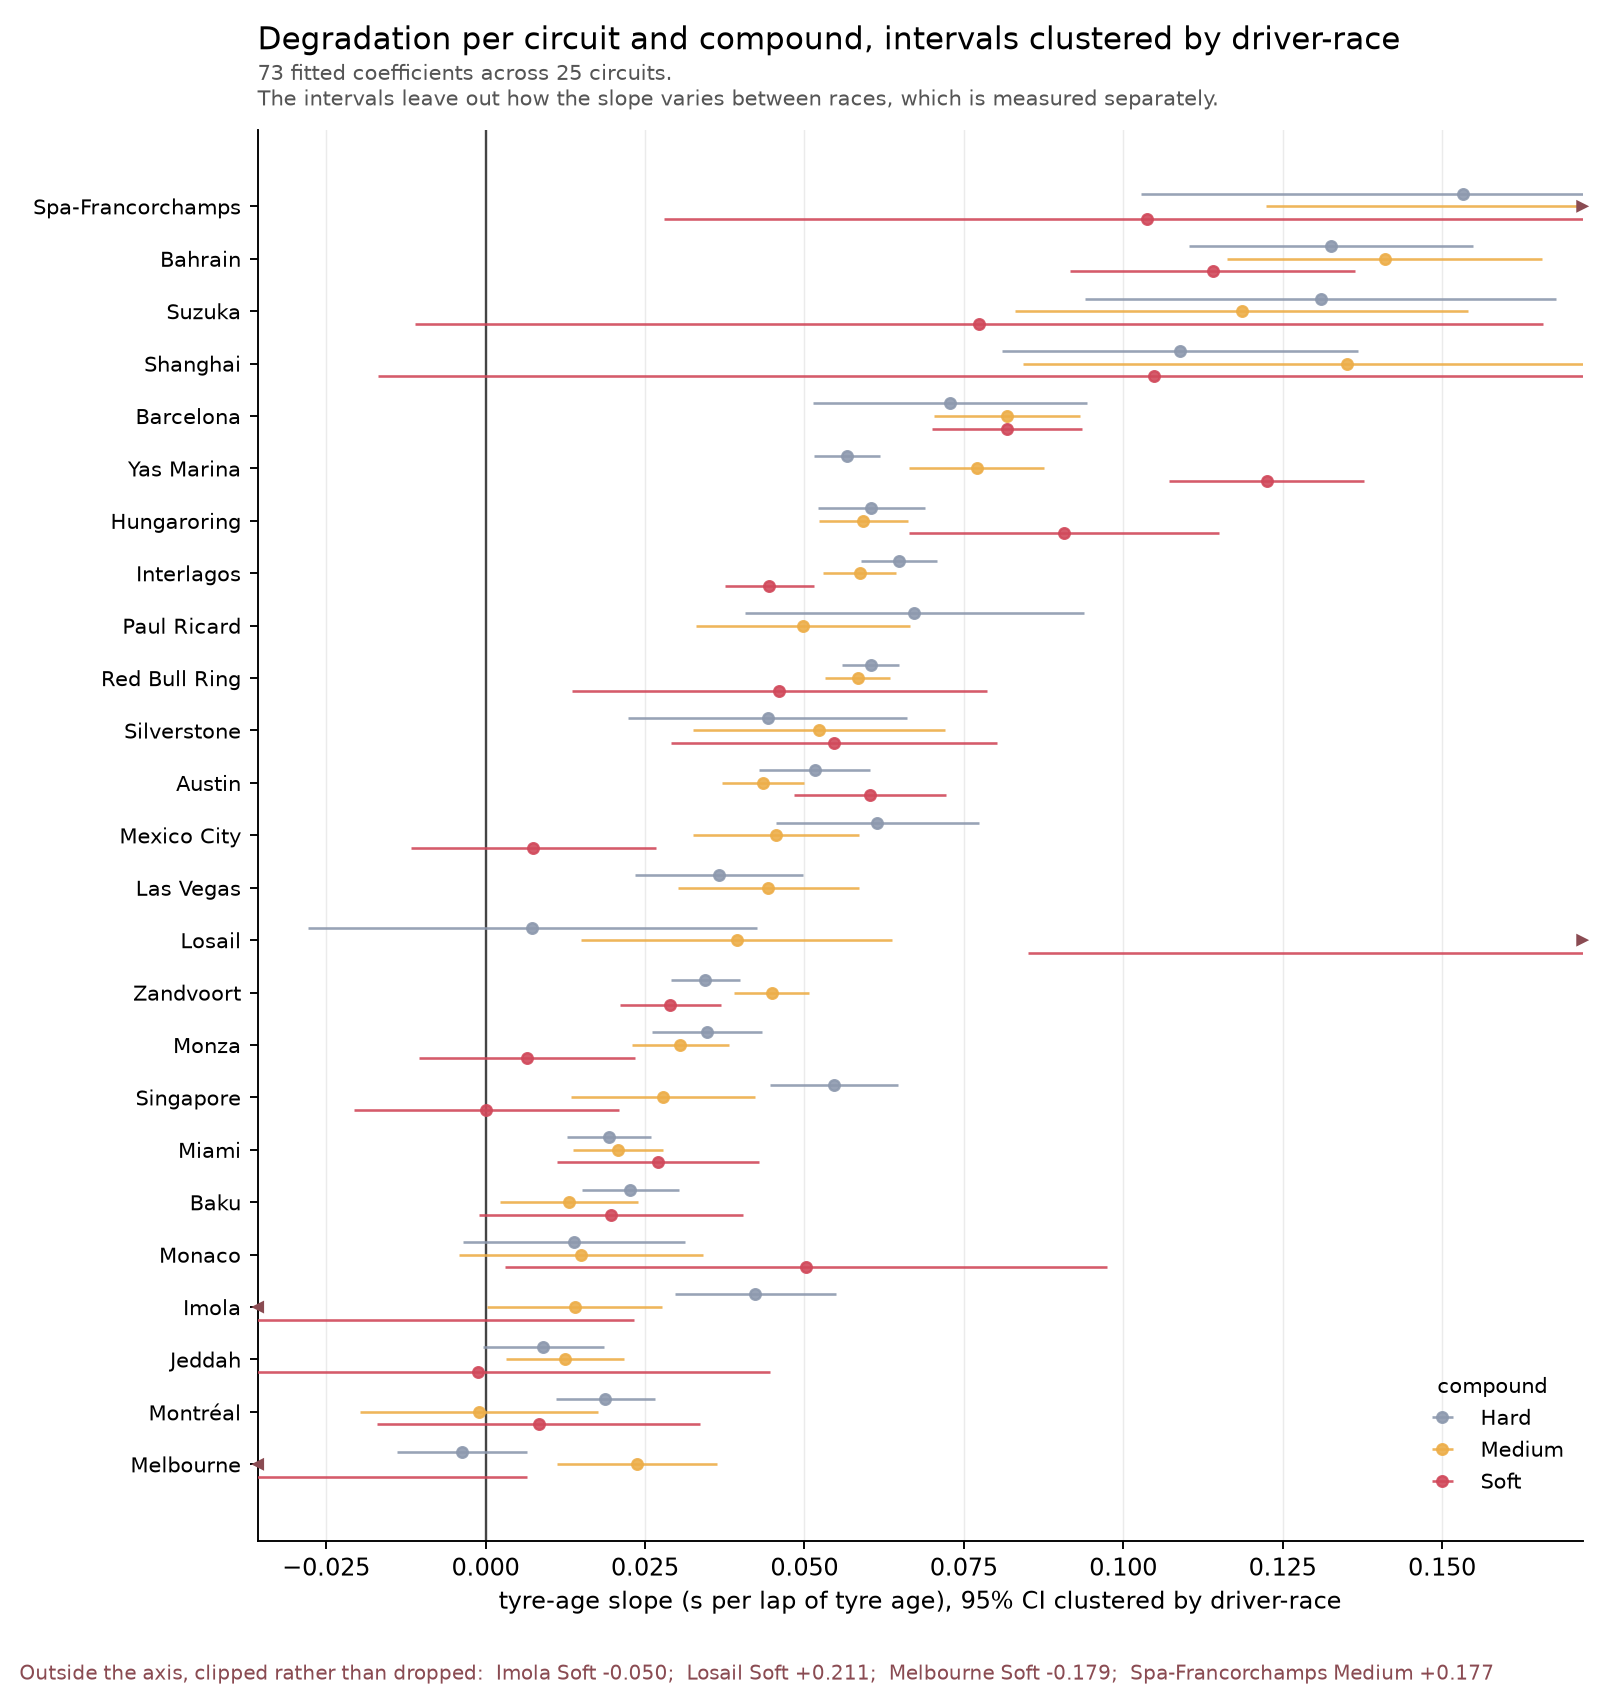
\includegraphics[width=0.82\textwidth]{s3_f1_degradation.png}
\caption{Coefficients linéaires de dégradation des pneus en Formule~1, par
circuit et par gomme, avec des intervalles groupés par pilote--course :
\NCoefficientsFone{} coefficients sur \NCircuitsFone{} circuits. Ces intervalles
n'incluent pas la variation de la pente entre courses, que la
Section~\ref{sec:variance} mesure. Les points hors de l'échelle tracée sont
nommés sous l'axe.}
\label{fig:degradation}
\end{figure}

Le modèle donne à chaque gomme sa propre pente d'usure mais pas de rythme de base
propre : une fois l'ordonnée pilote--course retirée, les gommes sont supposées
aussi rapides à neuf. La Section~\ref{sec:implied} teste ce que change un rythme
de base par gomme.

Deux caractéristiques de la Figure~\ref{fig:degradation} comptent pour la
suite. \PctCoefCrossingZero{}\,\% des pentes ont un intervalle qui contient zéro,
et à l'intérieur d'un circuit \PctCompoundOverlap{}\,\% des paires de gommes ont
des intervalles qui se chevauchent : la distinction entre gommes que porte le
modèle n'est en grande partie pas résolue par les données. Aucune des deux n'est
filtrée, parce que filtrer sur les pentes résolues sélectionnerait les circuits
les plus susceptibles de se transférer.

\subsection{Le transfert, et ce qui limite sa mesure}
\label{sec:transfermethod}

On ajuste sur toutes les saisons d'une catégorie-circuit sauf une, on prédit la
saison tenue à part, et on note le résidu centré dans chaque relais :
%
\begin{equation}
R^{2}_{\text{intra}} \;=\; 1 - \frac{\sum_{s}\sum_{\ell \in s}\bigl(\tilde{y}_{\ell} - \tilde{\hat{y}}_{\ell}\bigr)^{2}}{\sum_{s}\sum_{\ell \in s}\tilde{y}_{\ell}^{\,2}},
\qquad
\tilde{x}_{\ell} = x_{\ell} - \overline{x}_{s}.
\label{eq:transfer}
\end{equation}
%
Centrer chaque relais retire l'ordonnée pilote--course, qu'on ne peut pas
connaître pour une course qui n'a pas eu lieu, donc le score teste la
\emph{forme} que prend un relais. Comme $a$ et $\ell$ avancent ensemble dans un
relais, cette forme est le net de l'usure et du carburant : en Formule~1,
$(\beta_c + \phi)$ par tour. C'est sur cette quantité nette que porte le
Résultat~1, et sa taille limite ce qu'un score peut montrer.

\paragraph{Le plafond de bruit.} Un score faible a deux explications : la pente
a bougé entre saisons, ou il n'y a jamais eu assez de signal dans les tours pour
retrouver une pente. Pour les séparer, les temps au tour sont reconstruits à
partir de l'ajustement propre à chaque circuit avec \emph{une seule} pente de
dégradation pour toutes les saisons, donc une pente stable par construction, plus
des résidus rééchantillonnés par relais entiers pour garder leur corrélation
interne. Les résidus viennent d'un ajustement qui donne à chaque saison sa
propre pente, si bien qu'un vrai mouvement de la pente n'est pas compté comme du
bruit ; avec des résidus d'ajustement poolé, le plafond est plus bas d'au plus
\CeilingResidGapMax{} sur n'importe quel circuit. Faire tourner le vrai protocole
sur les tours reconstruits donne le plafond : le score qu'obtient une pente
parfaitement stable face au bruit présent. Un circuit est ensuite classé selon
le plafond et l'écart entre plafond et score mesuré : \emph{sans signal} si le
plafond est sous $\CeilingMeasurable{}$ ; sinon \emph{stable} si l'écart est sous
$\StableGap{}$, \emph{instable} s'il dépasse $\UnstableGap{}$, et \emph{limite}
entre les deux. Les ajustements synthétiques dégénérés sont exclus et nommés.

\paragraph{Variance entre courses.} Le plafond dit si le score pouvait détecter
un mouvement ; il ne mesure pas le mouvement. Pour cela, chaque circuit-gomme
reçoit une pente linéaire par saison, chaque saison étant une seule course, avec
son erreur-type groupée par pilote--course. La variance entre courses $\tau^2$
de ces pentes est estimée par maximum de vraisemblance restreint et par la
méthode des moments \citep{dersimonian1986},
avec un intervalle par profil de $Q$ \citep{viechtbauer2007}, et résumée par le
$Q$ de Cochran et par $I^2$, la part de la dispersion observée qui ne vient pas
de l'erreur d'échantillonnage \citep{higgins2002}. Comme les erreurs-types par
course ne tiennent pas compte des chocs communs à toutes les voitures au même
moment d'une course, $I^2$ est plutôt une borne haute. On fait de même pour
chaque catégorie-circuit d'endurance avec sa pente nette.

\subsection{Les planificateurs}
\label{sec:method}

\paragraph{Le programme dynamique multi-arrêts.} Pour une course d'endurance de
$L$ tours avec un rythme sous drapeau vert $p$, une pente nette $\beta$, une
perte au stand $\pi$ et une autonomie en carburant $F$, un plan est une
partition de $L$ en relais $(n_1,\dots,n_{m+1})$ avec $m$ arrêts, de temps total
%
\begin{equation}
T(n_1,\dots,n_{m+1}) \;=\; m\pi \;+\; \sum_{j}\left(n_j p + \beta\,\frac{n_j(n_j+1)}{2}\right),
\qquad n_j \le F,
\label{eq:dp}
\end{equation}
%
minimisé exactement par un programme dynamique sur les tours restants pour
chaque $m$ à partir du minimum imposé par le carburant,
$\lceil L/F \rceil - 1$. Une course est \emph{limitée par les pneus} quand le $m$
optimal en temps dépasse ce minimum.

\paragraph{Le moteur Monte Carlo.} Le moteur à arrêt suivant unique évalue
chaque tour candidat pour l'arrêt suivant sur \NDraws{} tirages partagés. Chaque
tirage échantillonne les coefficients de dégradation et de carburant dans leurs
lois d'échantillonnage ($t(G-1)$ mise à l'échelle des erreurs-types robustes aux
grappes), le taux de neutralisation dans sa loi a posteriori Gamma, et le bruit
des tours à l'échelle des résidus de validation croisée. Les tours candidats
partagent les tirages, donc une comparaison entre deux tours ne porte pas de
bruit d'échantillonnage étranger. Une variante \emph{attentive à la couverture}
fait tourner la voiture auditée et un rival sous les mêmes tirages, résout
l'échange au stand au tour où les deux se sont arrêtés, laisse survivre une
position gagnée avec le taux mesuré d'échanges entre voitures voisines sur le
circuit, et laisse le rival répondre à chaque tour de la voiture auditée par sa
meilleure réponse : un meneur de Stackelberg au sens de \citet{aguad2024},
résolu par énumération.

\subsection{L'audit}
\label{sec:auditprotocol}

\paragraph{Décisions.} Le moteur de la Section~\ref{sec:method} est le
planificateur audité. Pour chaque course avec un modèle ajusté, on rejoue le
premier arrêt de chacun des \NFinishers{} premiers classés en Formule~1
(\NCars{} voitures par catégorie en endurance). Le moteur est interrogé
\LookbackFone{} tours avant le vrai arrêt en Formule~1 et \LookbackEnd{} en
endurance, avec l'état tel qu'il était et les rivaux sur leurs vrais plans. Les
arrêts avant le tour \MinFirstStopFone{} (\MinFirstStopEnd{} en endurance) sont
exclus comme incidents. C'est une reconstitution, pas une prévision : le point
de décision est défini par un arrêt qui a eu lieu.

\paragraph{L'horizon engagé.} Le moteur planifie un arrêt. S'il a le droit de
mener le relais suivant jusqu'au drapeau, il répond à une autre question qu'une
équipe qui a déjà prévu un deuxième arrêt, et s'arrêtera plus tard pour cette
seule raison. Chaque décision dont le pilote s'est de nouveau arrêté est donc
rejouée avec une course qui se termine, pour le moteur, au vrai arrêt suivant de
ce pilote. Tout ce qui suit cet arrêt roule sur pneus neufs quel que soit le
tour choisi pour le premier arrêt, donc c'est commun à tous les candidats :
l'optimum sur l'horizon raccourci est l'optimum sachant l'arrêt suivant de
l'équipe. En endurance, chaque relais est aussi borné par l'autonomie en
carburant. Mené jusqu'au drapeau, le même moteur est en médiane \FoneMedian{}
tours en retard en Formule~1 ; ce chiffre est une propriété de la question, et
la Section~\ref{sec:audit} rapporte la reconstitution engagée.

\paragraph{Hors échantillon.} Les modèles de circuit sont ajustés sur les
saisons d'où viennent les décisions. Chaque décision engagée est donc aussi
rejouée avec les coefficients de carburant et de dégradation réajustés sur
toutes les saisons d'avant 2026 sauf la sienne, au degré publié ; un circuit
couru sur une seule saison ne peut pas être rejoué ainsi et est compté à part.

\paragraph{Règles de référence.} Avec un seul arrêt avant une fin fixée et des
pentes linéaires, l'arrêt optimal en temps $k$ tours après la décision vérifie
%
\begin{equation}
\beta_{\mathrm{old}}\,(a_0 + k) \;=\; \beta_{\mathrm{new}}\,(W - k),
\label{eq:closedform}
\end{equation}
%
pour un pneu d'âge $a_0$ et $W$ tours jusqu'à la fin. Elle ne dépend des pentes
que par leur rapport ; le terme de carburant et tout coût payé une fois par arrêt
s'annulent. Avec un rapport de un, elle équilibre l'âge des pneus de part et
d'autre de l'arrêt et n'utilise aucune quantité ajustée ; je l'appelle la
\emph{règle du rapport un}. Trois autres règles sont notées sur les décisions
menées jusqu'au drapeau : B1 divise la course en relais égaux ; B2 s'arrête
quand la perte accumulée du relais $\beta\,a(a+1)/2$ dépasse pour la première
fois la perte au stand ; B3 vide le réservoir, et n'est pas définie en
Formule~1, qui ne ravitaille plus depuis 2010.

\paragraph{Ce que révèlent les arrêts.} L'Équation~\ref{eq:closedform} peut être
inversée au tour choisi par l'équipe, ce qui donne le rapport
$\beta_{\mathrm{new}}/\beta_{\mathrm{old}} = (a_0+k)/(W-k)$ qui aurait rendu ce
tour optimal : l'âge du pneu à l'arrêt divisé par la longueur du relais
suivant. Aucune pente ajustée n'y entre. C'est un paramètre implicite, qui peut
représenter ce que les équipes savent ou ce qu'elles croient, et il utilise un
tour par décision. Un modèle de hasard en temps discret utilise
à la place chaque tour du relais : la probabilité de s'arrêter au tour $t$,
sachant que la voiture est encore en piste, est modélisée comme une fonction
logistique de la perte du vieux pneu au tour suivant $\hat\beta_{\mathrm{old}}a_t$
et de la perte du pneu neuf jusqu'à la fin $\hat\beta_{\mathrm{new}}(W-t)$, avec
les pentes ajustées introduites telles quelles et une indicatrice de tour
neutralisé. Le rapport des deux poids vaut un si les équipes pèsent les pneus
comme l'ajustement. À l'intérieur d'un relais, $a_t + (W-t)$ est constant, donc
les deux poids ne se distinguent que par la variation des pentes ajustées et de
$W$ entre relais ; le bruit des pentes fait donc partie de ce qui identifie le
rapport, et chaque réplication du bootstrap les réajuste sur les courses tirées.
$W$ est l'arrêt suivant de l'équipe, connu seulement après coup.

\paragraph{Intervalles.} Chaque intervalle est un bootstrap par percentiles au
niveau où les données varient : circuits ou catégories-circuits pour le
transfert, courses pour l'audit, puisque les pilotes d'une même course partagent
une piste, une voiture de sécurité et une allocation de pneus.

\begin{table}[htbp]
\centering
\caption{Chaque ensemble de décisions sur lequel un résultat est calculé. Tous
les ensembles de Formule~1 sont tirés des saisons d'avant le règlement 2026.}
\label{tab:samples}
\begin{tabular}{lrl}
\toprule
Ensemble de décisions & $n$ & Sert à \\
\midrule
Tous les premiers arrêts rejoués, quatre championnats & \NDecisions{} & Figure~\ref{fig:audit} \\
\quad notés par B1--B3 & \NScored{} & Tableau~\ref{tab:baselines} \\
Formule~1, cinq premiers, interrogés cinq tours avant & \NDecisionsFone{} & mené au drapeau \\
\quad rejouables avec l'arrêt suivant fixé & \NCommitAll{} & reconstitution engagée \\
\quad\quad courses à un arrêt & \NCommitOne{} & résidu \\
\quad\quad réajustés sans la saison & \OosN{} & hors échantillon \\
\quad entre deux gommes, circuits linéaires & \ImpliedN{} & rapport implicite, hasard \\
Formule~1, tous les classés, cinq tours avant & \DesignAllFiveN{} & vérifications de conception \\
Endurance, rejouables avec l'arrêt suivant fixé & \NEndCommit{} & reconstitution engagée \\
Formule~1, premiers arrêts sans neutralisation dans la fenêtre & \NDeviationCars{} & coût du résidu \\
\bottomrule
\end{tabular}
\end{table}

\section{Résultat 1 : le transfert n'est en général pas mesurable, et les pentes bougent bien}
\label{sec:transfer}

\begin{figure}[htbp]
\centering
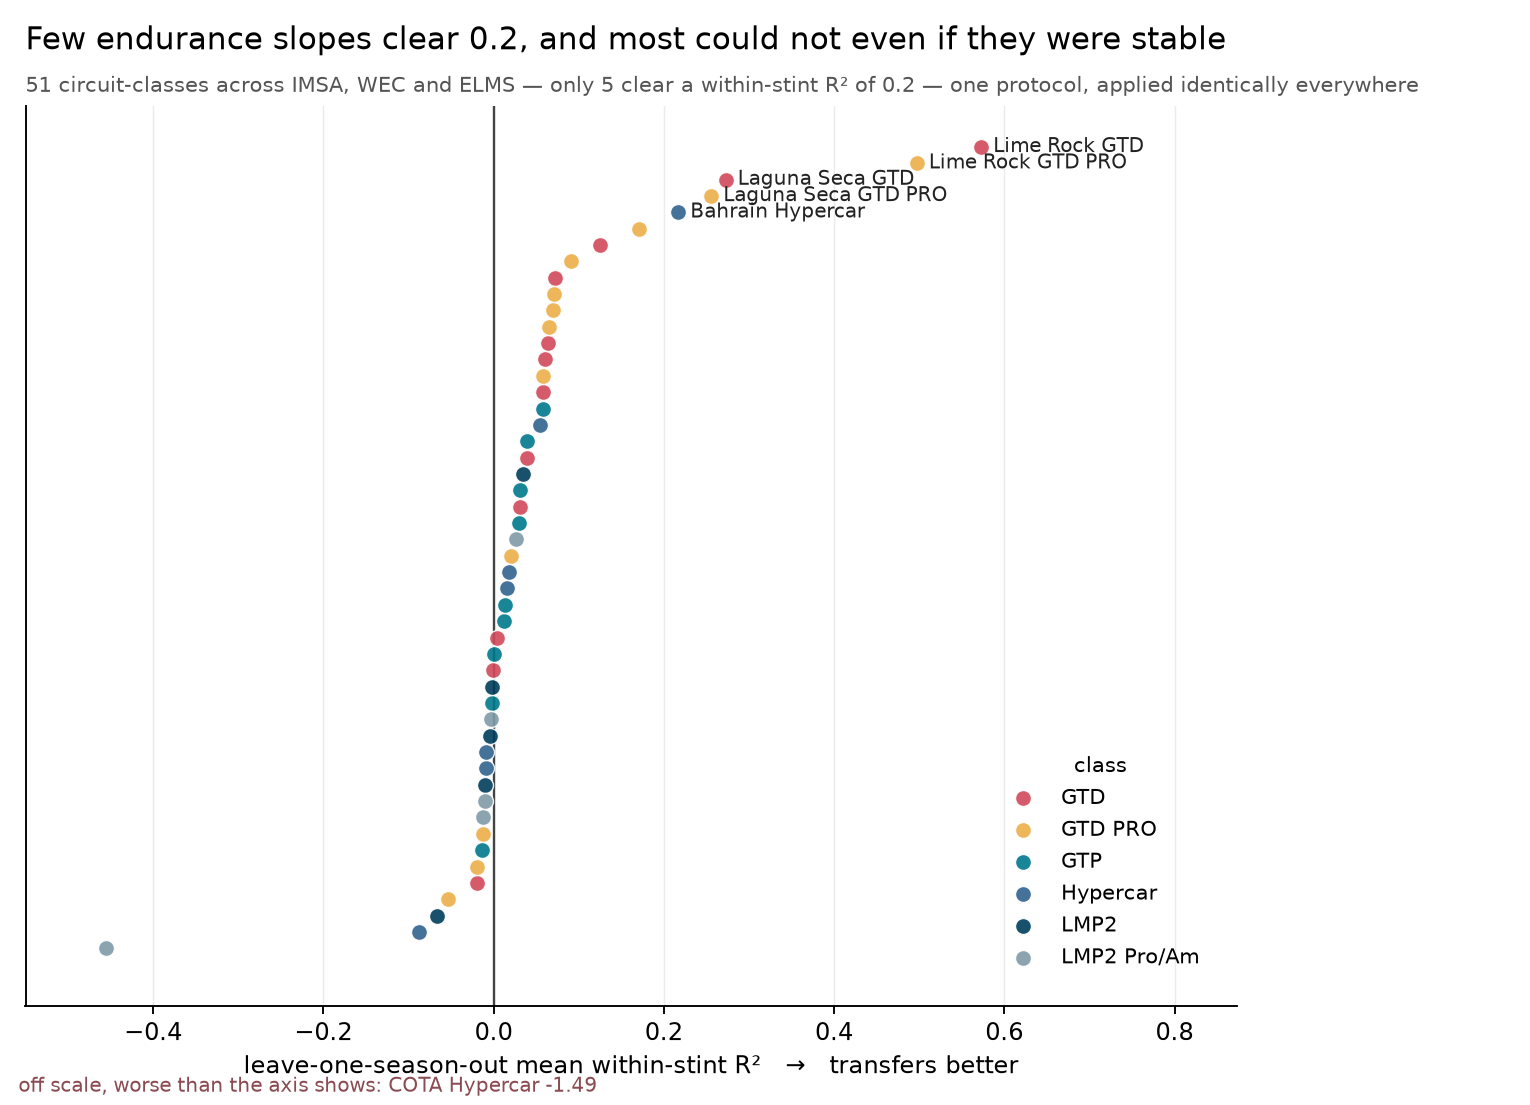
\includegraphics[width=0.86\textwidth]{r1_transfer.png}
\caption{$R^2$ intra-relais en laissant une saison de côté, un point par
catégorie-circuit d'endurance. Sur \NCircuitClasses{} mesurées,
\NTransferAboveTwo{} dépassent $\TransferThreshold{}$.}
\label{fig:transfer}
\end{figure}

Mesuré comme un décompte au-dessus d'un seuil, le transfert paraît rare. Sur
\NCircuitClasses{} catégories-circuits d'endurance, \NTransferAboveTwo{}
dépassent un $R^2$ intra-relais (Équation~\ref{eq:transfer}) de
$\TransferThreshold{}$ (Figure~\ref{fig:transfer}) ; le meilleur est
\BestTransfer{} à \BestTransferWhere{}, et presque partout ailleurs une pente
ajustée sur les autres saisons ne prédit pas la saison tenue à part mieux que la
propre moyenne de cette saison. La Formule~1 ressemble à cela :
\NFoneAboveTwo{} des \NCeilingCircuits{} circuits le dépassent. La suite de cette
section montre que le décompte parle surtout du signal, pas de la stabilité.

\subsection{Pourquoi le score est faible : carburant et usure s'annulent dans un relais}

Sur les \CancelN{} circuits de Formule~1 qui ont un verdict de plafond, le terme
médian en numéro de tour vaut \CancelFuel{}\,s par tour et la pente d'usure
médiane \CancelWear{} : dans un relais, la voiture gagne presque autant en
brûlant du carburant qu'elle perd sur ses pneus, et la pente nette que le score
doit prédire a une taille médiane de \CancelNet{}\,s par tour d'âge du pneu,
face à un bruit médian des tours de \CancelNoise{}\,s. À \CancelLowest{}, les
deux valent \CancelLowestFuel{} et \CancelLowestWear{}. La taille de la pente
nette classe les plafonds des circuits avec une corrélation de Spearman de
\CancelRho{}.

\begin{figure}[htbp]
\centering
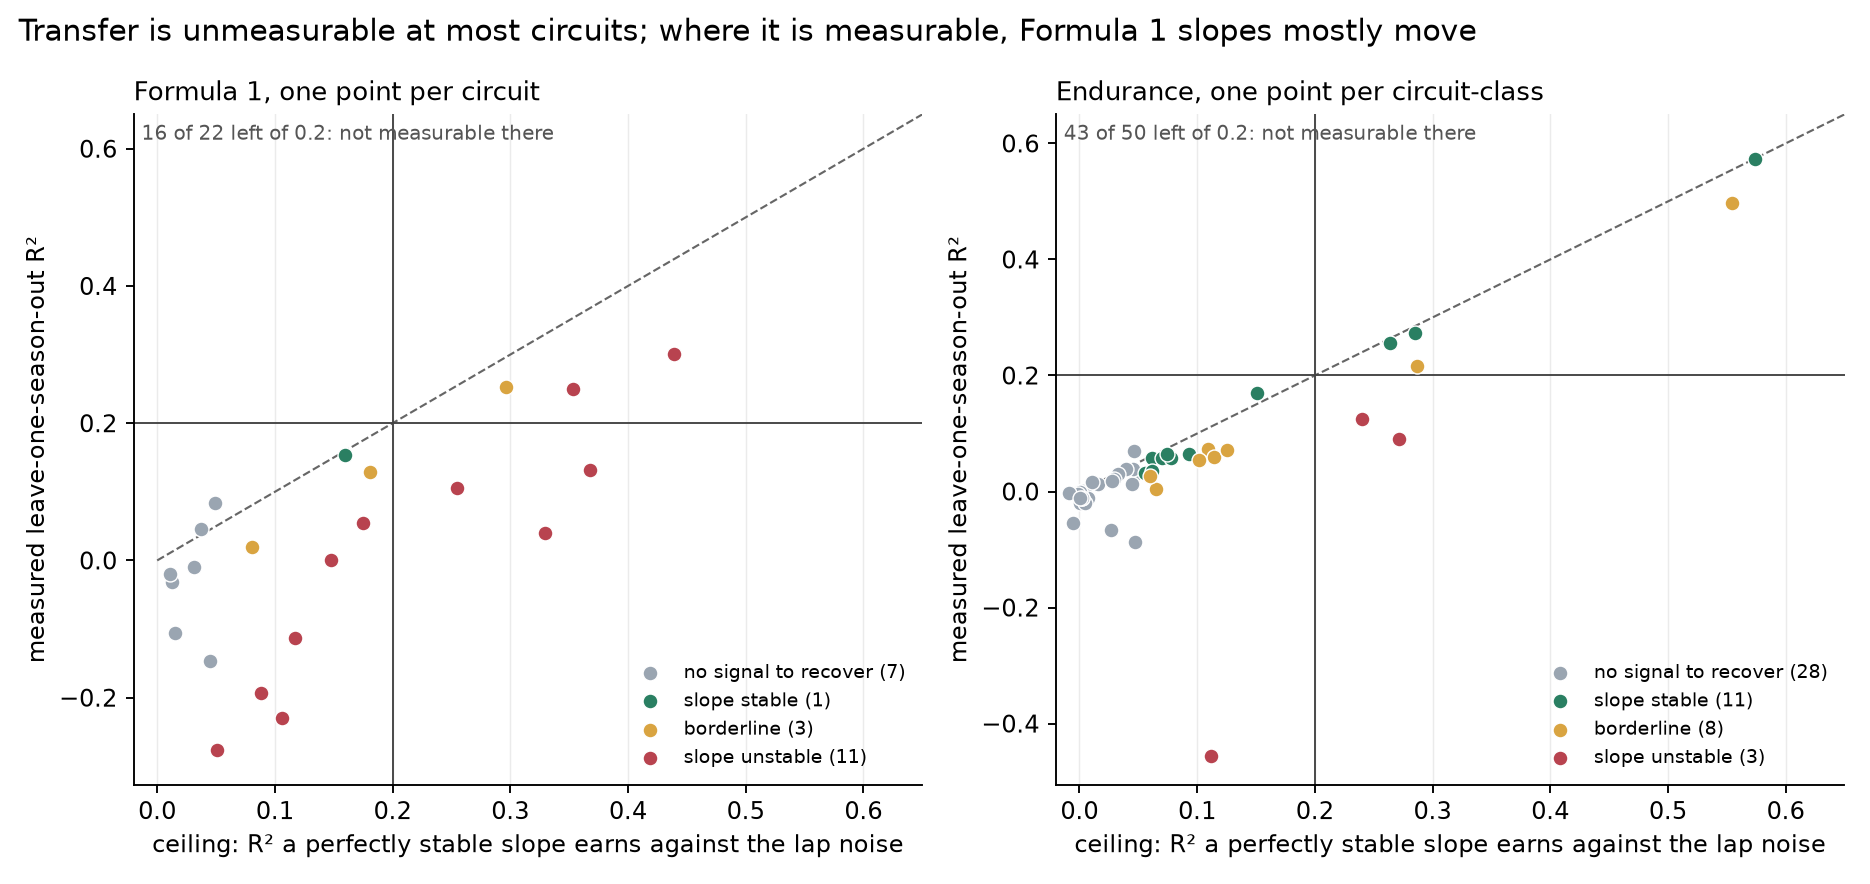
\includegraphics[width=\textwidth]{r1_ceiling.png}
\caption{Score mesuré en laissant une saison de côté, face au plafond qu'obtient
une pente parfaitement stable avec le même bruit des tours. Les points proches
de la diagonale en pointillés se transfèrent aussi bien qu'une pente stable le
pourrait ; les points bien en dessous ont des pentes qui bougent. À gauche de la
ligne verticale, aucune pente n'aurait pu dépasser $\TransferThreshold{}$.}
\label{fig:ceiling}
\end{figure}

Le plafond de bruit de la Section~\ref{sec:transfermethod} rend cela précis
(Figure~\ref{fig:ceiling}). Il va de \CeilingLowest{} à \CeilingLowestWhere{} à
\CeilingHighest{} à \CeilingHighestWhere{}, et sur \NCeilingBelowThreshold{}
des \NCeilingCircuits{} circuits de Formule~1 et \EndCeilBelow{} des
\EndCeilN{} catégories-circuits d'endurance, une pente parfaitement stable
n'aurait pas pu dépasser $\TransferThreshold{}$. Le décompte au-dessus du seuil
mesure donc au moins autant la quantité de signal d'un circuit que sa stabilité.

Rapportée à son plafond, la Formule~1 a \NCeilingUnstable{} circuits dont les
pentes bougent, \NCeilingStable{} dont la pente tient, \NCeilingNoSignal{} sans
signal récupérable et \NCeilingBorderline{} limites. Les catégories d'endurance
se répartissent autrement : \EndCeilNoSignal{} sans signal, \EndCeilStable{}
stables, \EndCeilBorderline{} limites et \EndCeilUnstable{} instables. Ces
données ne disent pas si ce contraste tient aux championnats ou au modèle, qui
porte une pente par gomme en Formule~1 et une pente nette en endurance.

\subsection{De combien la pente bouge entre courses}
\label{sec:variance}

Le plafond dit si le score aurait pu voir un mouvement ; les composantes de
variance le mesurent, sur la forme linéaire de l'Équation~\ref{eq:degradation}
ajustée saison par saison. Sur \VarN{} circuits-gommes de Formule~1 avec au
moins trois saisons, le $Q$ de Cochran rejette une pente commune pour \VarHet{}
d'entre eux, et l'$I^2$ médian vaut \VarIsq{} \VarIsqCi{} : l'essentiel de la
dispersion entre saisons n'est pas de l'erreur d'échantillonnage. L'écart-type
entre courses vaut une médiane de \TauPubShareReml{}\,\% \TauPubShareRemlCi{} de
la pente moyenne du circuit-gomme par maximum de vraisemblance restreint (REML),
\VarTauShare{}\,\% par l'estimateur des moments, qui sous-estime avec trois ou
quatre saisons, et son intervalle exclut zéro pour \VarTauExcl{} des \VarN{}.
Estimé comme un écart-type relatif commun aux \TauPubCommonN{} circuits-gommes
dont la moyenne est résolue, dans un modèle hiérarchique avec une moyenne
chacun, il vaut \TauPubCommon{}\,\% \TauPubCommonCi{}. $I^2$ est le plus haut là où le verdict du plafond dit instable (médiane
\VarIsqUnstable{}) et le plus bas là où il n'y a pas de signal
(\VarIsqNoSignal{}), donc les deux mesures concordent là où les deux peuvent
parler. En endurance, $Q$ rejette pour \EndVarHet{} des \EndVarN{}
catégories-circuits avec un $I^2$ médian de \EndVarIsq{}, dont \EndVarIsqStable{}
parmi celles que le plafond dit stables. Les pentes bougent entre courses presque
partout ; sur la plupart des circuits, le score intra-relais est simplement un
instrument trop faible pour s'en apercevoir.

Trois objections ne changent rien. \emph{Les étiquettes de gommes} : codées par
la gomme réelle de chaque tour, $Q$ rejette pour \TauRealHet{} des \TauRealN{}
et la part médiane vaut \TauRealShareReml{}\,\% \TauRealShareRemlCi{} ; sur les
\TauUnchangedCircuits{} circuits dont la désignation n'a jamais changé, pour
\TauUnchangedHet{} des \TauUnchangedN{}, avec une médiane de
\TauUnchangedShareReml{}\,\% \TauUnchangedShareRemlCi{}. Ce n'est pas un
changement de caoutchouc qui fait bouger la pente. \emph{La pente nette} :
saison par saison, la pente d'usure et le terme en numéro de tour se
compensent, donc la quantité que le score mesure vraiment est leur somme,
estimée directement en écrivant $\phi\ell + \beta a = \phi(\ell - a) +
(\beta + \phi)a$. Elle bouge davantage : $Q$ rejette pour \TauNetHet{} des
\TauNetN{}, avec un $I^2$ médian de \TauNetIsq{} et un écart-type entre courses
de \TauNetShareReml{}\,\% \TauNetShareRemlCi{} de sa moyenne.
\emph{L'estimateur} : les parts ci-dessus sont en REML ; l'estimateur des moments
donne des valeurs plus basses (\TauPubShareDl{}\,\% pour le codage publié,
\TauNetShareDl{}\,\% pour la pente nette), comme attendu avec trois ou quatre
saisons.

\paragraph{Température de piste.} La première cause candidate est la piste. En
régressant les pentes saisonnières sur la température de piste médiane de la
course, avec une ordonnée par circuit-gomme, on obtient \TempTheta{}\,s par tour
par dix degrés (erreur-type \TempThetaSe{}), face à un écart médian de
\TempRange{} degrés entre saisons sur un même circuit. L'effet est réel et
petit : il retire \TempShare{}\,\% de la variance entre courses.

Cette variance compte aussi pour l'audit. L'erreur-type à effets aléatoires de la
pente moyenne d'un circuit-gomme, qui compte la variation entre courses, vaut en
médiane \VarSeInflation{} fois celle groupée par pilote--course dans laquelle le
moteur tire, et jusqu'à \VarSeInflationMax{} fois. La Section~\ref{sec:audit}
refait l'audit avec ces lois élargies.

\subsection{Les réparations qu'une équipe essaierait}
\label{sec:repairs}

\paragraph{Coder le pneu par ce qu'il était.} Les noms de gommes sont relatifs :
Pirelli désigne trois de ses gommes pour chaque course, donc le Medium d'un même
circuit peut être un autre caoutchouc d'une saison à l'autre. J'ai relevé la
désignation pour les \NAllocationRaces{} courses de 2022 à 2025 dans les
articles Wikipédia de chaque course, vérifiée avec les communiqués de Pirelli
quand ils l'écrivent en texte (\NAllocationPirelli{} courses, en accord à chaque
fois), et recodé chaque tour. Là où l'allocation a changé, sur
\NCompoundChanged{} circuits qui ont un verdict de plafond, le score médian passe
de \CompoundRelative{} à \CompoundReal{}, une différence appariée de
\CompoundDiff{} \CompoundDiffCi{}, mieux sur \NCompoundBetter{} circuits et moins
bien sur \NCompoundWorse{}. Le recodage donne à chaque gomme réelle moins de
saisons que n'en avait son nom relatif, et ne répare pas le transfert.

\paragraph{La mesurer le vendredi.} En deuxième séance d'essais, chaque voiture
fait des relais longs sur les pneus et l'asphalte du week-end. Utilisée à la
place des autres saisons, la pente du vendredi obtient \FridayRaw{} contre
\FridayOther{}, moins bien sur \NFridayRawWorse{} des \NFridayRaces{} courses,
une différence appariée de \FridayRawDiff{} \FridayRawDiffCi{}. Les relais du
vendredi se dégradent plus vite que la course d'une médiane de
\FridayOffset{}\,s par tour ; retirer ce décalage, appris sur les autres
circuits, laisse encore \FridayCorrected{}.

\paragraph{Chiffrer la température.} Ajouter l'âge du pneu fois la température
de piste au modèle propre de chaque circuit, avec la température de la course
tenue à part, change le score d'une médiane de \TempOwnDiff{} \TempOwnDiffCi{} :
trois courses d'entraînement ne suffisent pas à fixer une sensibilité à la
température. Emprunter la sensibilité aux autres circuits le change plutôt de
\TempCatDiff{} \TempCatDiffCi{}, mieux sur \TempCatBetter{} des \TempN{}
circuits, trop peu pour l'établir.

\paragraph{Références.} Prédire chaque saison uniquement à partir des
précédentes, la question qu'une équipe se pose vraiment, coûte une médiane de
\BasePastDiff{} \BasePastDiffCi{} par rapport au fait de laisser une saison de
côté. Une pente commune à la catégorie, la médiane des ajustements de tous les
autres circuits, obtient \BaseCategoryDiff{} \BaseCategoryDiffCi{} par rapport à
celle du circuit : sur l'ensemble des circuits, l'historique d'un circuit ne bat
pas de façon mesurable une pente qui ne sait rien de lui. Sur les
\CeilingShareN{} circuits dont le plafond dépasse $\CeilingMeasurable{}$, la
pente propre au circuit retrouve une médiane de \CeilingShareMedian{} de son
plafond contre \CeilingShareCategory{} pour la pente de catégorie, une
différence de \CeilingCategoryDiff{} \CeilingCategoryDiffCi{} qui n'est pas
établie non plus. Réajustées avec le seuil de trafic à $\TrimLow{}$ ou
$\TrimHigh{}$ au lieu de $\TrimPublished{}$, au plus \TrimShareMoved{}\,\% des
pentes bougent de plus d'un dixième et le score médian va de \TrimLoroLow{} à
\TrimLoroHigh{} : les scores faibles dépendent du seuil de trafic, et aucun
réglage ne les approche de $\TransferThreshold{}$.

\subsection{Type de voiture}

Regroupés par type de voiture, les scores bruts favorisent les catégories GT3,
\GTThreeMean{} contre \ProtoMean{} pour les prototypes, une différence de
\TransferDiff{} \TransferDiffCI{} avec un $p$ de permutation de \TransferP{}.
Cette comparaison traite des catégories courant à des épreuves différentes comme
échangeables, et elles ne le sont pas : les deux meilleurs scores GT3, tous deux
à Lime Rock, viennent d'une épreuve sans catégorie prototype. Appariées dans les
\GtPairEvents{} épreuves qui ont les deux, les GT3 obtiennent un score plus haut
de \GtPairDiff{} \GtPairDiffCi{}, sur \GtPairHigher{} d'entre elles, avec un $p$
exact par changement de signe de \GtPairP{}. La différence brute est surtout une
différence entre circuits, et je n'en revendique pas entre types de voiture.
Pour la même raison, le plateau ELMS LMP2, presque monotype, ne peut rien dire de
la Balance of Performance : sur \NLmptwoNoSignal{} de ses \NLmptwoTotal{}
circuits, ses tours ne portent aucun signal récupérable.

\section{Une note sur le planificateur d'endurance}
\label{sec:regime}

Le programme dynamique de l'Équation~\ref{eq:dp} indique aussi, pour chaque
course d'endurance, si le plan optimal pour les pneus demande plus d'arrêts que
le minimum imposé par le carburant : \NTyreLimited{} des \NRaceSeasons{}
courses-saisons le demandent. Le régime est décidé à l'intérieur du
planificateur en comparant un arrêt de plus à ce que le pneu rend, donc c'est
presque une identité du modèle, et il n'est rapporté ici que comme une
description de la position de ces championnats. Classées par la seule perte au
stand, les courses-saisons se séparent avec une AUC de \RegimeAucPitLoss{}
\RegimeAucPitLossCI{}, par la seule pente nette à \RegimeAucSlope{}
\RegimeAucSlopeCI{} ; retirer l'un ou l'autre de l'indice propre au
planificateur, $\log\beta + 2\log n - \log\pi$, coûte un montant semblable
(\IndexDropDiff{} \IndexDropDiffCi{}), donc les deux fixent le régime. Le
ravitaillement fait une médiane de \RefuelShare{}\,\% de la perte à l'arrêt et
ne change pas le décompte, et aucune course-saison limitée par les pneus n'a une
perte au-dessus de \CheapStopEdge{}\,s, une limite fixée par une course. La
Figure~\ref{fig:pitloss} en annexe montre la relation au niveau des catégories
($r = \PitLossR{}$ sur six points de catégorie). La décision que les équipes
d'endurance prennent le plus souvent, changer ou non les pneus à un arrêt
carburant, n'est pas dans le modèle (Section~\ref{sec:threats}).

\section{Résultat 2 : avec la stratégie tenue fixe, le planificateur s'accorde avec les équipes, et l'accord vient de l'horizon}
\label{sec:audit}

Le planificateur choisit le tour de l'arrêt suivant pour minimiser le temps de
course attendu d'une voiture, sur les décisions et les horizons de la
Section~\ref{sec:auditprotocol}. Il ne représente ni l'allocation de pneus, ni le
trafic, ni la gestion de l'énergie, ni une position au championnat. Chaque
chiffre ci-dessous mesure un désaccord entre un modèle et une pratique, pas ce
qui était le plus rapide.

\begin{figure}[htbp]
\centering
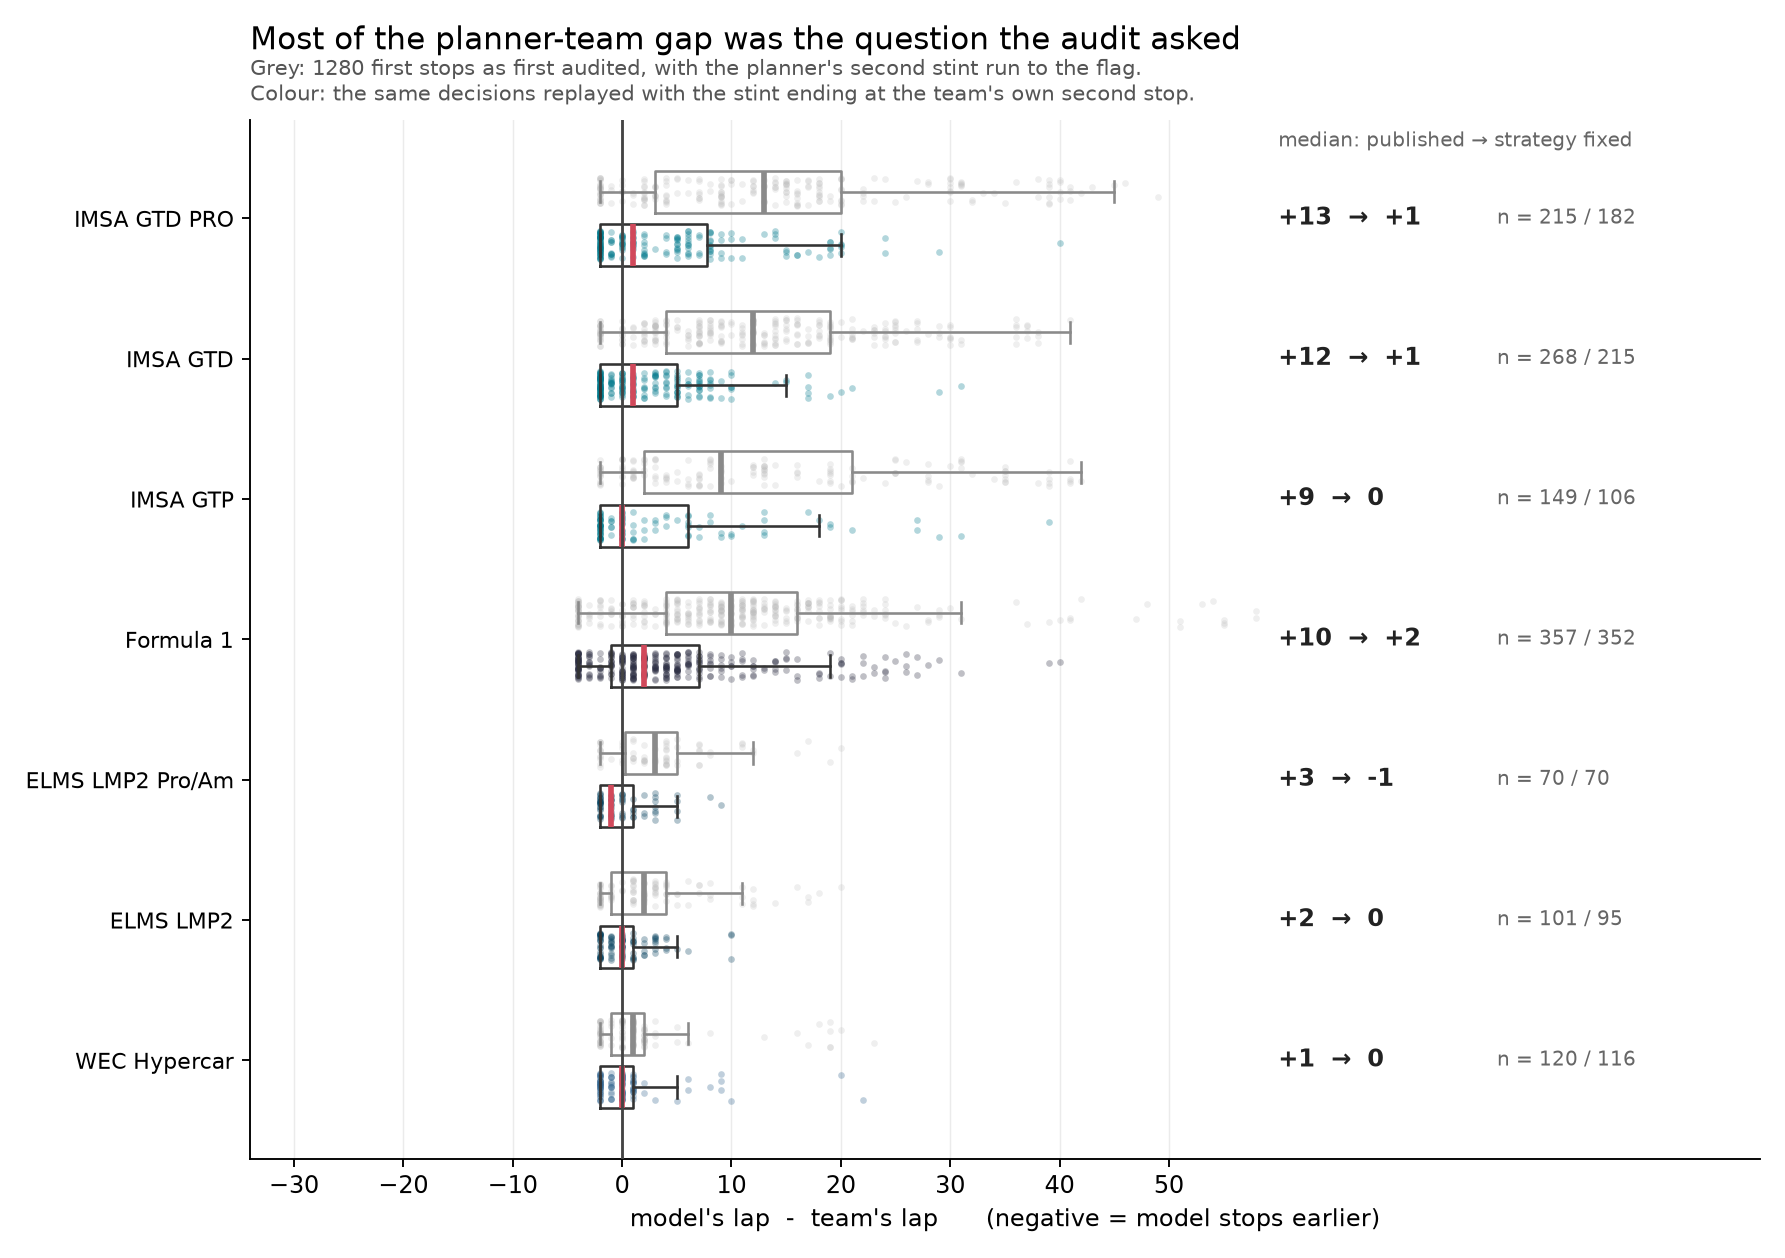
\includegraphics[width=\textwidth]{r3_audit_bias.png}
\caption{Tour du modèle moins tour de l'équipe sur les \NDecisions{} premiers
arrêts rejoués. Gris : le moteur mené jusqu'au drapeau. Couleur : les mêmes
décisions avec un relais qui se termine au propre arrêt suivant de l'équipe ;
en endurance, seules les décisions avec un arrêt ultérieur peuvent être
rejouées. Les boîtes montrent les quartiles.}
\label{fig:audit}
\end{figure}

\subsection{L'accord}
\label{sec:committed}

Avec l'arrêt suivant de chaque équipe tenu fixe, le planificateur tombe à une
médiane de \CommitAllAfter{} tours \CommitAllCi{} du vrai arrêt sur les
\NCommitAll{} décisions de Formule~1 rejouables, contre \CommitAllBefore{} quand
les mêmes décisions sont menées jusqu'au drapeau (Figure~\ref{fig:audit}). En
endurance, l'intervalle contient zéro dans les \NEndCommitContainsZero{}
catégories.

L'accord résiste aux vérifications qu'un lecteur demanderait d'abord.
\begin{itemize}
\item \emph{Hors échantillon.} Avec des pentes ajustées sans la saison de la
décision, la médiane est de \OosMedian{} \OosCi{} sur \OosN{} décisions, contre
\OosPublished{} dans l'échantillon sur les mêmes ; le tour recommandé bouge pour
\OosMoved{}\,\% des décisions, d'une médiane de \OosShift{} tour.
\item \emph{Incertitude élargie.} Avec la loi d'échantillonnage de chaque pente
élargie à son erreur-type à effets aléatoires, la médiane est de \WideMedian{}
\WideCi{}.
\item \emph{Conception.} Interrogé dix ou quinze tours avant au lieu de cinq, et
sur tous les classés au lieu des cinq premiers, la médiane va de
\DesignMinMedian{} à \DesignMaxMedian{} sur six conceptions.
\item \emph{Drapeau vert seulement.} Sur les \FoneGreenN{} décisions dont le vrai
arrêt a eu lieu sous drapeau vert, elle est de \FoneGreenMedian{}
\FoneGreenCi{} ; en ne gardant que les décisions dont l'arrêt \emph{suivant} a
eu lieu sous drapeau vert, \CommitGreenAfter{} \CommitGreenCi{}. En IMSA, où
\ImsaCautionMin{} à \ImsaCautionMax{}\,\% des premiers arrêts sont pris sous
neutralisation, les médianes sous drapeau vert sont \ImsaGtpGreenMedian{},
\ImsaGtdGreenMedian{} et \ImsaGtdproGreenMedian{} pour GTP, GTD et GTD PRO.
\item \emph{Pas une fenêtre étroite.} Dans les courses de Formule~1 avec un
deuxième arrêt, la fenêtre entre la décision et cet arrêt fait une médiane de
\CommitWindow{} tours ; un tour tiré uniformément dans cette fenêtre manquerait
le vrai arrêt d'une médiane de \CommitUniformMiss{} et le milieu de la fenêtre
de \CommitMidpointMiss{}, contre \CommitEngineMiss{} pour le moteur sur les
mêmes décisions. En endurance, le moteur ne bat les deux que dans les
\NEndCommitInformative{} catégories IMSA ; en WEC Hypercar et en ELMS,
l'autonomie en carburant laisse \EndCommitWecHypercarWindow{} à
\EndCommitElmsLmptwoProAmWindow{} tours et la reconstitution n'est pas
informative.
\end{itemize}

Conditionner sur l'arrêt suivant de l'équipe, c'est conditionner sur une décision
ultérieure, prise en sachant où avait eu lieu le premier arrêt. La médiane
engagée est un accord sachant le plan que l'équipe a révélé, ce qui fait que le
planificateur et l'équipe répondent à la même question ; ce n'est pas une mesure
de la qualité du planificateur.

\subsection{D'où vient l'accord}
\label{sec:designchecks}

L'Équation~\ref{eq:closedform} décrit ce que fait le moteur : elle tombe à une
médiane de \ClosedFormGap{} tour du tour du moteur sur \ClosedFormN{} décisions
sur circuits linéaires. Sa forme à rapport un, qui n'utilise aucune quantité
ajustée, est la référence naturelle, et elle égale l'erreur absolue médiane du
moteur dans \RatioOneTies{} catégories sur \RatioOneClasses{}
(Tableau~\ref{tab:baselines}). L'accord de la reconstitution engagée est donc
produit par l'horizon : une fois l'arrêt suivant de l'équipe connu, équilibrer
l'âge des pneus avant lui est aussi proche de la pratique que le moteur complet.
Sur cette mesure, le Monte Carlo, le hasard de neutralisation et les pentes
ajustées n'ajoutent rien à l'accord.

En endurance, c'est forcé. Le modèle a une seule pente nette, donc
$\beta_{\mathrm{old}} = \beta_{\mathrm{new}}$, le choix du tour se réduit à des
âges de pneus égaux de part et d'autre de l'arrêt quelle que soit la pente, et la
reconstitution teste la logique de carburant et de neutralisation plutôt que le
modèle de pneus.

\begin{table}[htbp]
\centering
\caption{Erreur absolue médiane en tours face au vrai arrêt, par catégorie. Les
quatre premières colonnes sont menées jusqu'au drapeau, sur les \NScored{}
décisions que les règles peuvent noter ; les deux dernières reçoivent l'arrêt
suivant de l'équipe, sur les décisions que la reconstitution engagée peut
traiter. En gras, le meilleur des quatre premiers.}
\label{tab:baselines}
\begin{tabular}{lrrrrrr}
\toprule
& \multicolumn{4}{c}{Mené au drapeau} & \multicolumn{2}{c}{Arrêt suivant fixé} \\
\cmidrule(lr){2-5}\cmidrule(lr){6-7}
& Optimiseur & B1 & B2 & B3 & Optimiseur & Rapport un \\
\midrule
Formule~1        & \FoneModelError{}            & \FoneBoneError{}            & \textbf{\FoneBtwoError{}}   & \FoneBthreeError{} & \FoneCommitError{} & \FoneRatioOneError{} \\
IMSA GTP         & \ImsaGtpModelError{}         & \ImsaGtpBoneError{}         & \ImsaGtpBtwoError{}         & \ImsaGtpBthreeError{} & \ImsaGtpCommitError{} & \ImsaGtpRatioOneError{} \\
IMSA GTD         & \ImsaGtdModelError{}         & \textbf{\ImsaGtdBoneError{}}     & \ImsaGtdBtwoError{}    & \ImsaGtdBthreeError{} & \ImsaGtdCommitError{} & \ImsaGtdRatioOneError{} \\
IMSA GTD PRO     & \ImsaGtdproModelError{}      & \textbf{\ImsaGtdproBoneError{}}  & \ImsaGtdproBtwoError{} & \ImsaGtdproBthreeError{} & \ImsaGtdproCommitError{} & \ImsaGtdproRatioOneError{} \\
WEC Hypercar     & \WecHypercarModelError{}     & \WecHypercarBoneError{}     & \WecHypercarBtwoError{}     & \textbf{\WecHypercarBthreeError{}} & \WecHypercarCommitError{} & \WecHypercarRatioOneError{} \\
ELMS LMP2        & \textbf{\ElmsLmptwoModelError{}} & \ElmsLmptwoBoneError{}  & \ElmsLmptwoBtwoError{}      & \ElmsLmptwoBthreeError{} & \ElmsLmptwoCommitError{} & \ElmsLmptwoRatioOneError{} \\
ELMS LMP2 Pro/Am & \ElmsLmptwoProAmModelError{} & \textbf{\ElmsLmptwoProAmBoneError{}} & \ElmsLmptwoProAmBtwoError{} & \ElmsLmptwoProAmBthreeError{} & \ElmsLmptwoProAmCommitError{} & \ElmsLmptwoProAmRatioOneError{} \\
\bottomrule
\end{tabular}
\end{table}

Mené jusqu'au drapeau, une règle empirique est plus proche de la pratique que
l'optimiseur dans \NClassesRuleWins{} catégories sur \NClassesScored{}, et dans
\NClassesBoneWins{} d'entre elles la règle est B1, qui n'utilise aucune quantité
ajustée. Sachant l'arrêt suivant de l'équipe, l'optimiseur est plus proche que
toutes les règles dans \NClassesCommitBeatsRules{} catégories et égale la
meilleure dans \NClassesCommitTiesRules{}, mais la règle du rapport un, sachant
le même arrêt suivant, fait aussi bien. L'avantage des règles sur l'optimiseur
mené au drapeau venait de la question posée à cet optimiseur.

\subsection{Le résidu}
\label{sec:residual}

Ce qui reste est concentré dans les courses à un arrêt, où le planificateur et
l'équipe répondaient depuis le début à la même question : \CommitOneAfter{} tours
\CommitOneCi{} sur \NCommitOne{} décisions, \OosOneMedian{} \OosOneCi{} hors
échantillon. Une partie tient à la fenêtre de l'audit. Interrogé cinq tours avant
l'arrêt, le planificateur peut être au plus quatre tours en avance et en retard
sans limite, et \DesignTopFiveBound{}\,\% des décisions engagées sont sur cette
borne ; rejouée pour tous les classés quinze tours avant, la médiane à un arrêt
est de \DesignAllFifteenOneMedian{} \DesignAllFifteenOneCi{}. Une partie tient à
l'extrapolation : \ExtrapOne{}\,\% des recommandations à un arrêt s'arrêtent à un
âge de pneu au-delà du 95\textsuperscript{e} centile des relais observés sur
cette gomme à ce circuit, là où la pente linéaire n'est plus mesurée, et quand la
recommandation reste dans cette plage, la médiane à un arrêt est de
\ExtrapOneInsideGap{}. Ce que cela coûte est traité à la
Section~\ref{sec:deviationcost}.

\subsection{Ce que révèlent les arrêts}
\label{sec:implied}

Le résidu a une forme qui ne dépend pas de la fenêtre. Inverser
l'Équation~\ref{eq:closedform} au tour choisi par chaque équipe, sur les
\ImpliedN{} décisions entre deux gommes différentes sur circuits linéaires,
donne un rapport médian $\beta_{\mathrm{new}}/\beta_{\mathrm{old}}$ de
\ImpliedRatio{} \ImpliedRatioCi{} contre \ImpliedFitted{} ajusté. Comme le
rapport implicite vaut $(a_0+k)/(W-k)$, cela dit d'abord que les premiers relais
des équipes sont plus courts que les relais qui les suivent ; la valeur ajustée
à laquelle on le compare est un rapport que les ajustements ne résolvent pas,
puisque \PctCompoundOverlap{}\,\% des paires de gommes se chevauchent.

Le sens du changement sépare les deux lectures. Si les équipes agissent sur une
différence entre gommes que les ajustements manquent, le rapport implicite doit
tomber sous un quand elles passent à une gomme plus dure et dépasser un quand
elles passent à une gomme plus tendre ; si autre chose raccourcit les premiers
relais, il doit tomber sous un dans les deux cas. Il se sépare selon la dureté
(Tableau~\ref{tab:direction}) : vers une gomme plus dure, le rapport implicite
vaut \ImpliedHarder{} \ImpliedHarderCi{} sur \ImpliedHarderN{} décisions, vers
une plus tendre \ImpliedSofter{} \ImpliedSofterCi{} sur \ImpliedSofterN{}
décisions dans \ImpliedSofterRaces{} courses, et il est du côté de un que
prévoit la dureté pour \ImpliedExpectedSide{}\,\% des décisions. Les rapports
ajustés le sont pour \ImpliedFittedExpectedSide{}\,\%, pas mieux qu'une pièce :
ils placent la gomme plus dure à \ImpliedFittedHarder{} de l'usure de la plus
tendre, et la plus tendre à \ImpliedFittedSofter{} de celle de la plus dure. Le
rapport implicite mesure donc ce que l'ajustement ne résout pas : les équipes
s'arrêtent comme si elles savaient quelle gomme dure, et de combien, et
l'ajustement publié ne le montre pas. Une partie de cela est le même savoir
exercé dans l'autre sens, choisir la gomme plus dure pour le relais plus long,
que l'inversion ne peut pas distinguer d'un rythme d'usure. Le \ImpliedRatio{}
poolé est surtout le cas vers une gomme plus dure, qui est le cas courant.

Une partie de ce que l'ajustement manque tient à sa propre spécification.
Réajusté avec un rythme de base par gomme, la gomme plus dure est plus lente à
neuf, de \OffsetHarder{}\,s \OffsetHarderCi{} sur les décisions qui passent à
elle, et les pentes réajustées rangent les gommes du côté attendu pour
\OffsetsFittedSide{}\,\% des décisions au lieu de \ImpliedFittedExpectedSide{}\,\% :
mieux que le hasard, encore loin des équipes. Avec ces rythmes de base dans
l'arrêt unique optimal en temps, le tour du planificateur passe de
\OffsetsGapPlain{} à \OffsetsGap{} tours \OffsetsGapCi{} de celui de l'équipe,
donc les premiers relais plus courts demeurent.

\begin{table}[htbp]
\centering
\caption{Rapports implicite et ajusté $\beta_{\mathrm{new}}/\beta_{\mathrm{old}}$
selon le sens du changement de gomme, décisions de Formule~1 entre deux gommes
différentes sur circuits linéaires. Les intervalles rééchantillonnent les
courses.}
\label{tab:direction}
\begin{tabular}{lrrll}
\toprule
Changement & Décisions & Courses & Rapport implicite & Rapport ajusté \\
\midrule
Vers une gomme plus dure & \ImpliedHarderN{} & \ImpliedHarderRaces{} & \ImpliedHarder{} \ImpliedHarderCi{} & \ImpliedFittedHarder{} \ImpliedFittedHarderCi{} \\
Vers une gomme plus tendre & \ImpliedSofterN{} & \ImpliedSofterRaces{} & \ImpliedSofter{} \ImpliedSofterCi{} & \ImpliedFittedSofter{} \ImpliedFittedSofterCi{} \\
\bottomrule
\end{tabular}
\end{table}

Le modèle de hasard d'arrêt, ajusté sur les \HazardLaps{} tours où ces
\HazardStints{} premiers relais étaient exposés, place le poids que les équipes
donnent à la perte ajustée du pneu neuf, par rapport à celle du vieux pneu, à
\HazardRatio{} \HazardRatioCi{} avec les pentes réajustées à chaque réplication
(\HazardRatioCiFixed{} si on les tient fixes). Il s'accorde avec le rapport
implicite en signe, pas en taille, et il ne peut pas séparer les deux sens :
\HazardHarder{} \HazardHarderCi{} vers une gomme plus dure, \HazardSofter{}
\HazardSofterCi{} vers une plus tendre. Comme il n'est identifié qu'entre
relais, par des pentes qui ne résolvent pas les gommes et une fin connue
seulement après coup, je le lis comme compatible avec le rapport implicite
plutôt que comme une deuxième mesure de celui-ci.

Le savoir sur les gommes n'est pas la seule chose que le paramètre implicite
peut absorber : une usure qui s'accélère en fin de relais, la valeur de garder
l'option d'une voiture de sécurité et la gestion des pneus vers une longueur de
relais prévue agissent toutes sur le même rapport. Cinq autres mécanismes que
j'ai pu tester n'expliquent pas les premiers relais plus courts :
\begin{itemize}
\item \emph{Une usure qui croît avec la charge de carburant.} Un terme âge du
pneu fois numéro de tour a un signe variable, positif sur \InterPositive{} des
\InterN{} circuits, et refaire l'Équation~\ref{eq:closedform} avec lui fait
passer l'écart médian de \InterGapWithout{} à \InterGapWith{} tours, en
s'éloignant du vrai arrêt.
\item \emph{Des premiers relais plus lourds.} Ajustées séparément, les pentes du
premier relais ne sont plus raides que celles des suivants que sur
\FirstSteeper{} des \FirstPairs{} circuits-gommes, et des \FirstSig{} différences
significatives, \FirstSigSteeper{} vont dans ce sens ; les utiliser fait passer
l'écart de \FirstGapPooled{} à \FirstGapSplit{} tours, là aussi en s'éloignant.
\item \emph{La position en piste.} Le moteur attentif à la couverture rapproche la
recommandation du vrai arrêt sur \RetestCloser{} des \NRetest{} décisions à un
arrêt et l'en éloigne sur \RetestFurther{}, et sous chacune des \NRetestRules{}
règles de choix du rival ci-dessous, il la rapproche sur au plus
\RetestCloserMax{} (test du signe $p \le \RetestSignPMax{}$).
\item \emph{Le premier undercut indéfendable} de \citet{salminen2026}, avec la
défense qui conserve la position, ne prédit aucun undercut indéfendable avant le
drapeau sur \NRetestEuuAfterFlag{} des \NRetestPredicted{} décisions à un arrêt
qui portent une prédiction. Sur les \NRetestEuuInside{} où son tour tombe pendant
la course, son erreur absolue dépasse celle de l'optimiseur à une voiture d'une
médiane de \RetestEuuInsideAbsDiff{} tours \RetestEuuInsideAbsDiffCi{}, plus
proche sur \RetestEuuInsideCloser{} et plus loin sur \RetestEuuInsideFurther{}.
Sur toutes les décisions de Formule~1, pour qu'il reproduise ce que font les
équipes, les pneus devraient s'user d'une médiane de \DOneImpliedTheta{}\,s par
tour, \DOneThetaRatio{} fois le rythme mesuré.
\item \emph{Un gain à l'arrêt.} Avec un nombre d'arrêts fixé, tout temps gagné ou
perdu une fois par arrêt est commun à tous les tours candidats et s'annule ; il
ne peut pas déplacer le tour. Les données montrent d'ailleurs un tel terme de
signe opposé : les tours sur un train neuf sont plus lents que ce que prévoit
l'ajustement, ce qui est la mise en température.
\end{itemize}
Une pente biaisée vers la durabilité agirait dans le bon sens ; face à un
historique de tours indépendant au schéma Ergast, distribué sur Kaggle, qui sépare
l'usure du carburant par une autre méthode, la différence appariée médiane sur
\CrossSourceN{} circuits est de \CrossSourceDiff{}\,s par tour face à une pente
d'usure médiane de \CrossSourceWear{}. Une estimation structurelle complète à la
manière de \citet{rust1987}, avec la différence entre gommes comme paramètre et
non comme entrée ajustée, est l'endroit où l'explication du rapport commencerait.

\subsection{Ce que coûte le résidu}
\label{sec:deviationcost}

Le planificateur chiffre le résidu à quelques dixièmes de seconde. Sur le même
morceau de chaque vraie course, de la décision à l'arrêt suivant ou au drapeau,
fenêtres neutralisées retirées, j'ai comparé le temps écoulé de chaque voiture à
ce que prédit son propre tour médian sous drapeau vert, à l'intérieur des courses
et en contrôlant la longueur de la fenêtre. Sur \NDeviationCars{} premiers arrêts
dans \NDeviationRaces{} courses, chaque tour d'écart avec le tour du
planificateur va avec \DeviationPerLap{}\,s de temps en plus
\DeviationPerLapCi{}, contre \DeviationPlannerPerLap{}\,s selon le propre prix du
planificateur. Entre voitures d'une même course, le temps en excès a un
écart-type médian de \DeviationSpread{}\,s, donc le plus petit coût par tour que
ces décisions pourraient détecter avec une puissance de 80\,\% est d'environ
\DeviationMde{}\,s, et détecter le propre prix du planificateur demanderait
environ \DeviationNeeded{} décisions. C'est une association entre voitures,
ouverte à toutes les raisons qu'une équipe avait pour son tour.

\subsection{Quelle voiture est le rival}
\label{sec:rivalchoice}

Un modèle attentif à la concurrence a besoin d'un rival, et le chronométrage
n'en nomme pas. La reconstitution publiée associe chaque voiture à sa voisine la
plus proche au classement, ce qui, comme l'a fait remarquer Charles Thraves,
choisit la voiture devant pour certaines décisions et la voiture derrière pour
d'autres. Face à cela, j'ai fait tourner sa proposition (la voiture dont le temps
de course optimal seul est le plus proche), la voiture devant au chronomètre sur
laquelle est défini le modèle de \citet{salminen2026}, et toute voiture à moins
d'une perte au stand. Sur les \NRivalAllApply{} décisions où les \NRivalRules{}
s'appliquent, elles nomment la même voiture \NRivalAllAgree{} fois ; deux à deux,
deux règles s'accordent sur \RivalPairMin{} à \RivalPairMax{}\,\% des décisions,
une médiane de \RivalPairMedian{}\,\%. La recommandation bouge à peine entre
elles : le moteur attentif à la couverture reste plus tard que le vrai arrêt sous
chaque règle. La littérature de théorie des jeux repose sur une abstraction à
deux voitures \citep{aguad2024,devries2026,salminen2026} ; face à de vraies
décisions, quelles sont ces deux voitures est sous-déterminé.

\section{Menaces sur la validité}
\label{sec:threats}

\paragraph{L'horizon engagé est rétrospectif.} La reconstitution de la
Section~\ref{sec:committed} reçoit l'arrêt suivant de l'équipe. Se limiter aux
arrêts suivants sous drapeau vert retire les arrêts opportunistes, pas un plan
révisé pendant la course.

\paragraph{L'horloge des pneus en endurance.} Les équipes d'endurance font
souvent un double relais sur les mêmes pneus, et la décision à laquelle elles
font face est souvent de changer ou non les pneus à un arrêt carburant. Le
modèle d'endurance compte l'âge du pneu à partir de l'estimation de la source,
porte une seule pente nette sans gomme, et ne représente pas cette décision ;
son régime limité par les pneus répond à une question que les équipes
d'endurance se posent rarement, et sa reconstitution ne peut pas tester le
modèle de pneus (Section~\ref{sec:designchecks}).

\paragraph{Les pentes dépendent de la stratégie.} Un pilote à qui l'on demande de
faire durer un train le ménage, donc une pente ajustée dépend en partie du relais
que l'équipe a choisi, ce qui pousse dans le sens du résidu à un arrêt et
apparaîtrait entre saisons comme de l'instabilité. Le chronométrage public ne
peut pas le retirer.

\paragraph{Réutiliser, pas réajuster.} Comme l'a dit Giona Fieni, une politique
fondée sur un modèle réajuste ses courbes de dégradation pour chaque voiture et
chaque circuit et ne dépend jamais du transfert d'une pente. Le Résultat~1 borne
les approches qui reportent des paramètres ajustés (Section~\ref{sec:transfer}) ;
pour une conception qui réajuste systématiquement, c'est un argument pour
réajuster.

\paragraph{Décidé après avoir vu les données.} La reconstitution engagée, la
correction du rival, les vérifications de conception et les analyses des
Sections~\ref{sec:variance}, \ref{sec:residual} et \ref{sec:implied}, y compris
la séparation du rapport implicite selon le sens, ont toutes été construites
après avoir vu l'écart mené au drapeau. La protection contre un
chemin bifurquant est un test que l'analyse n'a pas pu voir, gelé à la
Section~\ref{sec:prospective}.

\paragraph{Estimateurs retirés et constantes fragiles.} Une base par morceaux en
temps de course, destinée à absorber l'évolution de la piste, a été retirée après
avoir échoué sur de vrais plateaux, dont l'identifiabilité médiane de
\NIdentifiability{} sort de la plage où elle avait été montrée efficace. Les
meilleurs scores de transfert en endurance reposent sur deux ou trois plis
chacun. Les deux sont documentés dans le dépôt.

\section{Reproductibilité et test prospectif}
\label{sec:reproducibility}

Chaque artefact dérivé des données commitées est régénéré par l'intégration
continue, qui échoue à la moindre différence entre l'arbre de travail et le dépôt.
Chaque nombre de ce manuscrit est une macro générée à partir des artefacts
commités ; la source ne contient aucun chiffre en propre. L'état à partir duquel
les résultats ont été calculés est archivé sur Zenodo, à
\url{https://doi.org/10.5281/zenodo.22726130}. Le dépôt ne redistribue pas les
deux exports tiers, tous deux téléchargés sur Kaggle, que lisent
\NBlockedLayers{} de ses couches : un historique de Formule~1 au schéma Ergast
(temps au tour, arrêts, résultats) et une table de résultats WEC. Ces couches ne
peuvent pas être régénérées à partir d'un clone ; leurs sorties sont commitées, et
le seul résultat publié qui en dépend est la vérification croisée des pentes de
la Section~\ref{sec:implied}.

\paragraph{Un test prospectif, gelé avant que ses données existent.}
\label{sec:prospective}
La reconstitution engagée --- planificateur, graines, recul, sélection des
voitures et horizon --- est gelée dans \texttt{paper/prospective\_protocol.md},
commité avant que les courses de Formule~1 sur lesquelles il sera noté aient eu
lieu, avec ses hypothèses et ses intervalles de prédiction fixés à l'avance : une
médiane engagée dans \ProspectivePiSeason{} tours sur la saison complète suivante
et, comme test secondaire sur les courses restantes de la saison en cours, dans
\ProspectivePiFour{}. Deux hypothèses ajoutées avant la première de ces courses
ne dépendent pas du recul : tout le plateau rejoué quinze tours avant, et le
rapport implicite. Les modèles gelés ont été ajustés sur des voitures construites
selon le règlement précédent, donc le test demande aussi si la reconstitution
survit à un changement de règlement. Le résultat sera rapporté face au fichier
daté, quel qu'il soit. L'hypothèse cinq gèle le rapport implicite poolé, dont la
valeur dépend de la part des changements vers une gomme plus dure ; la
séparation du Tableau~\ref{tab:direction} est venue après le gel et n'en fait
pas partie.

\paragraph{Les courses de 2026 déjà récupérées.} Les \HeldIngested{} Grands Prix
de 2026 déjà présents dans le dépôt ont été récupérés avant le gel du test et
sont tenus hors de tout modèle de ce papier. L'audit n'avait jamais tourné sur
eux ; leurs tours sont entrés dans une première version du plafond de bruit,
avant qu'il soit limité à 2022--2025. Rejoués avec les modèles gelés, hors
échantillon mais \emph{non} pré-enregistrés, les \HeldRaces{} qui ont une
décision rejouable donnent une médiane engagée de \HeldMedian{} tours \HeldCi{}
sur \HeldN{} décisions, \HeldWideMedian{} \HeldWideCi{} pour tout le plateau
quinze tours avant sur \HeldWideN{} décisions, et un rapport implicite de
\HeldImplied{} \HeldImpliedCi{} sur \HeldImpliedN{} décisions, toutes vers une
gomme plus dure, contre \ImpliedHarder{} dans ce sens en 2022--2025. L'accord
engagé survit au changement de règlement. Le rapport implicite est plus proche
de un sur les nouvelles voitures et les nouveaux pneus, mais sur
\HeldImpliedN{} décisions son intervalle atteint la valeur de 2022--2025, donc
aucun changement n'est établi.

\section{Conclusion}

Le chronométrage public contient rarement assez de signal pour dire si une pente
de dégradation se transfère, et la raison est physique : à l'intérieur d'un
relais, le carburant brûlé annule presque l'usure du pneu, donc la forme d'un
relais est petite face au bruit des tours. Mesurée directement, la pente bouge
entre courses presque partout, d'une médiane de \TauPubShareReml{}\,\% de sa
moyenne, et d'environ sa propre taille pour la pente nette que montre un
relais ; ni un changement de gomme ni la température de piste n'en expliquent
beaucoup. Tenu à la stratégie engagée de l'équipe, et hors échantillon, un
planificateur qui minimise le temps s'arrête à quelques tours du muret des
stands, mais une règle qui se contente d'équilibrer l'âge des pneus avant
l'arrêt suivant de l'équipe aussi : l'accord est une propriété de l'horizon. Ce
que les arrêts révèlent, c'est la différence entre gommes que l'ajustement
manque. Lue comme un rapport d'usure implicite, la longueur du premier relais
d'une équipe face au suivant suit la dureté des gommes dans les deux sens de
changement, là où les pentes ajustées ne font pas mieux que le hasard, et
seulement un peu mieux quand chaque gomme a son propre rythme de base. Les
équipes agissent comme si elles savaient quel pneu dure ; le chronométrage
public, tel que modélisé ici, ne le montre qu'en partie.

\section*{Disponibilité des données et du code}

Chaque quantité de ce papier est dérivée d'artefacts commités par des scripts
d'un dépôt public (Section~\ref{sec:reproducibility}), qui contient aussi les
données, les figures et les tests :
\url{https://github.com/mohammedmedjadj/Motorsport-Strategy-Lab}. L'état à partir
duquel les résultats ont été calculés est archivé à
\url{https://doi.org/10.5281/zenodo.22726130}.

\section*{Remerciements}

Plusieurs chercheurs ont répondu à des e-mails non sollicités sur ce travail, et
leurs réponses l'ont changé. Charles Thraves (Universidad de Chile) a identifié le
défaut de choix du rival, proposé la règle du temps seul de la
Section~\ref{sec:rivalchoice}, et nommé l'endogénéité qui la borne. Wytze de
Vries (TU Eindhoven) a soulevé deux objections de mesure au régime d'endurance
de la Section~\ref{sec:regime} : que les
médianes de catégorie mélangent des arrêts avec et sans changement de pilote, et
qu'une partie de la corrélation pourrait aller dans l'autre sens ; les deux ont
été testées, et aucune ne dérange l'ordre des catégories. Jorn van Kampen (TU
Eindhoven) a décrit la même structure en endurance électrique, où un changement
de pneus est négligeable à côté de l'arrêt de recharge. Giona Fieni (ETH Z\"urich)
a tracé la ligne entre paramètres réutilisés et politique fondée sur un modèle
reprise à la Section~\ref{sec:threats}. Felipe Carrasco Heine a fait remarquer
que le modèle de temps au tour n'a pas de rythme de base par gomme, ce que teste
la Section~\ref{sec:implied}. Aucun d'eux n'est responsable de ce que dit ce
manuscrit.

\appendix
\section{Le coût de l'arrêt dans le planificateur d'endurance}

\begin{figure}[htbp]
\centering
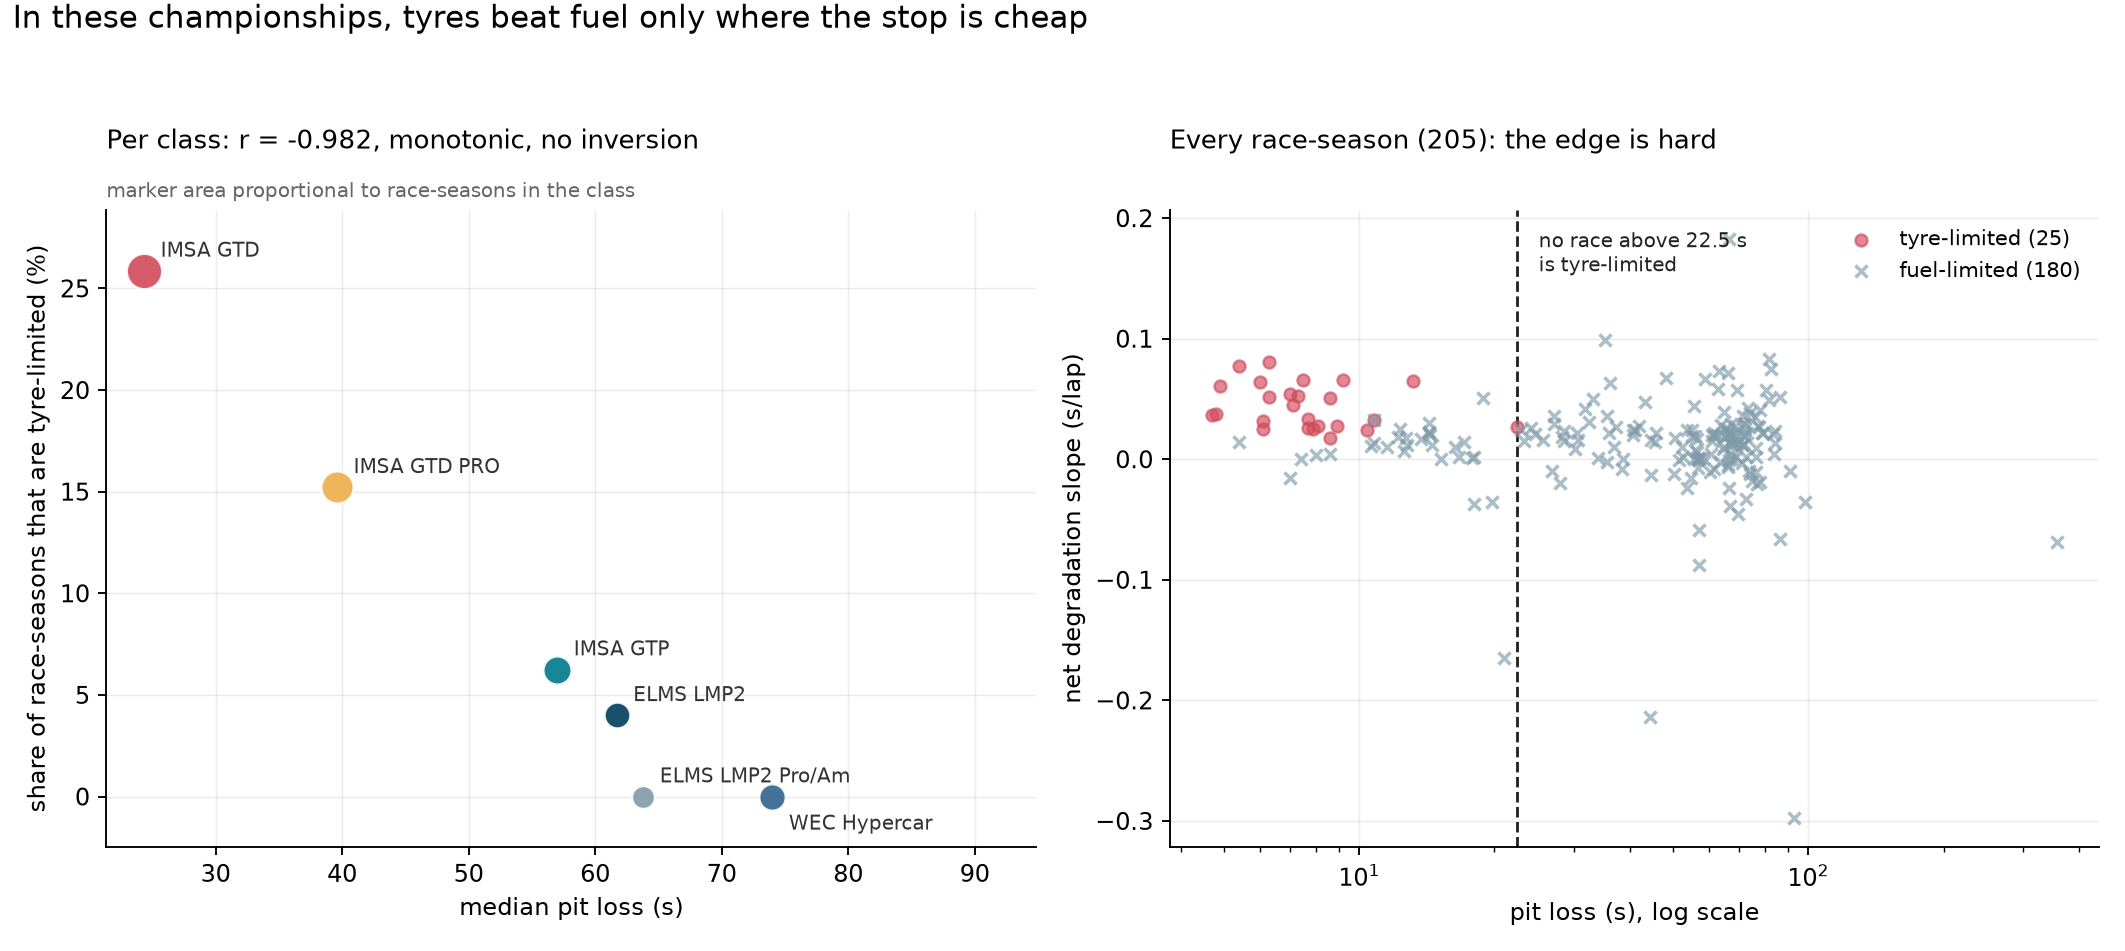
\includegraphics[width=\textwidth]{r2_pit_loss_rule.png}
\caption{À gauche : perte au stand médiane par catégorie face à la part des
courses-saisons dont le plan optimal pour les pneus demande plus d'arrêts que le
minimum imposé par le carburant. À droite : chaque course-saison, avec la limite
empirique marquée (Section~\ref{sec:regime}).}
\label{fig:pitloss}
\end{figure}

\begin{thebibliography}{99}

% APA 7th, which the journal's submission guidelines require. Every entry was
% checked against a publication record -- Crossref for the journal articles,
% the arXiv API for the preprints, the Zenodo API for the one deposited there
% -- rather than recalled from memory. Two candidate references carried in
% earlier notes could not be confirmed and are deliberately absent. One entry
% has not been peer reviewed by anyone and its own line says so, which is the
% only honest way to cite it. See reports/cross_series/related_work.md.

\bibitem[Aguad and Thraves(2024)]{aguad2024}
Aguad, F., \& Thraves, C. (2024). Optimizing pit stop strategies in Formula 1
with dynamic programming and game theory. \emph{European Journal of
Operational Research}, \emph{319}(3), 908--919.
\url{https://doi.org/10.1016/j.ejor.2024.07.011}

\bibitem[Bekker and Lotz(2009)]{bekker2009}
Bekker, J., \& Lotz, W. (2009). Planning Formula One race strategies using
discrete-event simulation. \emph{Journal of the Operational Research Society},
\emph{60}(7), 952--961.
\url{https://doi.org/10.1057/palgrave.jors.2602626}

\bibitem[Boettinger and Klotz(2023)]{boettinger2023}
Boettinger, M., \& Klotz, D. (2023). \emph{Mastering Nordschleife: A
comprehensive race simulation for AI strategy decision-making in motorsports}
(arXiv:2306.16088). arXiv. \url{https://arxiv.org/abs/2306.16088}

\bibitem[Cameron and Miller(2015)]{cameron2015}
Cameron, A.~C., \& Miller, D.~L. (2015). A practitioner's guide to
cluster-robust inference. \emph{Journal of Human Resources}, \emph{50}(2),
317--372.

\bibitem[Cappello and Hoegh(2026)]{cappello2026}
Cappello, C., \& Hoegh, A. (2026). A state-space approach to modeling tire
degradation in Formula 1 racing. \emph{Journal of Sports Analytics},
\emph{12}. \url{https://doi.org/10.1177/22150218261446170}

\bibitem[Carrasco Heine and Thraves(2022)]{carrasco2022}
Carrasco Heine, O.~F., \& Thraves, C. (2022). On the optimization of pit stop
strategies via dynamic programming. \emph{Central European Journal of
Operations Research}, \emph{31}(1), 239--268.
\url{https://doi.org/10.1007/s10100-022-00806-4}

\bibitem[DerSimonian and Laird(1986)]{dersimonian1986}
DerSimonian, R., \& Laird, N. (1986). Meta-analysis in clinical trials.
\emph{Controlled Clinical Trials}, \emph{7}(3), 177--188.
\url{https://doi.org/10.1016/0197-2456(86)90046-2}

\bibitem[de~Vries et~al.(2026)]{devries2026}
de Vries, W., van den Eshof, E., van Kampen, J., \& Salazar, M. (2026).
\emph{Competitor-aware race management for electric endurance racing}
(arXiv:2603.28286). arXiv. \url{https://arxiv.org/abs/2603.28286} (Accepted for
presentation at IEEE ITSC 2026)

\bibitem[Fieni et~al.(2025)]{fieni2025}
Fieni, G., W\"uthrich, J., Neumann, M.-P., Moradi, M.~M., \& Onder, C.~H.
(2025). \emph{Towards learning-based Formula 1 race strategies}
(arXiv:2512.21570). arXiv. \url{https://arxiv.org/abs/2512.21570}

\bibitem[Fieni et~al.(2026)]{fieni2026}
Fieni, G., W\"uthrich, J., Neumann, M.-P., \& Onder, C.~H. (2026).
\emph{Learning-based multi-agent race strategies in Formula 1}
(arXiv:2602.23056). arXiv. \url{https://arxiv.org/abs/2602.23056}

\bibitem[Heilmeier et~al.(2018)]{heilmeier2018}
Heilmeier, A., Graf, M., \& Lienkamp, M. (2018). A race simulation for strategy
decisions in circuit motorsports. In \emph{2018 21st International Conference
on Intelligent Transportation Systems (ITSC)} (pp. 2986--2993).
\url{https://doi.org/10.1109/ITSC.2018.8570012}

\bibitem[Heilmeier et~al.(2020a)]{heilmeier2020mc}
Heilmeier, A., Graf, M., Betz, J., \& Lienkamp, M. (2020). Application of Monte
Carlo methods to consider probabilistic effects in a race simulation for
circuit motorsport. \emph{Applied Sciences}, \emph{10}(12), 4229.
\url{https://doi.org/10.3390/app10124229}

\bibitem[Heilmeier et~al.(2020b)]{heilmeier2020nn}
Heilmeier, A., Thomaser, A., Graf, M., \& Betz, J. (2020). Virtual strategy
engineer: Using artificial neural networks for making race strategy decisions
in circuit motorsport. \emph{Applied Sciences}, \emph{10}(21), 7805.
\url{https://doi.org/10.3390/app10217805}

\bibitem[Higgins and Thompson(2002)]{higgins2002}
Higgins, J.~P.~T., \& Thompson, S.~G. (2002). Quantifying heterogeneity in a
meta-analysis. \emph{Statistics in Medicine}, \emph{21}(11), 1539--1558.
\url{https://doi.org/10.1002/sim.1186}

\bibitem[Romer(2006)]{romer2006}
Romer, D. (2006). Do firms maximize? Evidence from professional football.
\emph{Journal of Political Economy}, \emph{114}(2), 340--365.
\url{https://doi.org/10.1086/501171}

\bibitem[Rust(1987)]{rust1987}
Rust, J. (1987). Optimal replacement of GMC bus engines: An empirical model of
Harold Zurcher. \emph{Econometrica}, \emph{55}(5), 999--1033.
\url{https://doi.org/10.2307/1911259}

\bibitem[Salminen(2026)]{salminen2026}
Salminen, T. (2026). \emph{Game-theoretic framework for pit stop strategy
optimisation in circuit auto racing}. Zenodo.
\url{https://doi.org/10.5281/zenodo.21306419} (Preprint, single author, not
peer reviewed)

\bibitem[Santillana(2026)]{santillana2026}
Santillana, J.~S. (2026). \emph{Pitwall: Faithful natural-language
race-strategy briefings from a calibrated real-time Monte Carlo engine}
(arXiv:2607.06495). arXiv. \url{https://arxiv.org/abs/2607.06495}

\bibitem[Thomas et~al.(2025)]{thomas2025}
Thomas, D., Jiang, J., Kori, A., Russo, A., Winkler, S., Sale, S., McMillan,
J., Belardinelli, F., \& Rago, A. (2025). \emph{Explainable reinforcement
learning for Formula One race strategy} (arXiv:2501.04068). arXiv.
\url{https://arxiv.org/abs/2501.04068}

\bibitem[Todd et~al.(2025)]{todd2025}
Todd, J., Jiang, J., Russo, A., Winkler, S., Sale, S., McMillan, J., \& Rago,
A. (2025). \emph{Explainable time series prediction of tyre energy in Formula
One race strategy} (arXiv:2501.04067). arXiv.
\url{https://arxiv.org/abs/2501.04067}

\bibitem[Tulabandhula and Rudin(2014)]{tulabandhula2014}
Tulabandhula, T., \& Rudin, C. (2014). Tire changes, fresh air, and yellow
flags: Challenges in predictive analytics for professional racing. \emph{Big
Data}, \emph{2}(2), 97--112. \url{https://doi.org/10.1089/big.2014.0018}

\bibitem[van Kampen et~al.(2022)]{vankampen2022}
van Kampen, J., Herrmann, T., \& Salazar, M. (2022). Maximum-distance race
strategies for a fully electric endurance race car. \emph{European Journal of
Control}, \emph{68}, 100679.
\url{https://doi.org/10.1016/j.ejcon.2022.100679}

\bibitem[van Kampen et~al.(2024)]{vankampen2024}
van Kampen, J., Moriggi, M., Braghin, F., \& Salazar, M. (2024). \emph{Model
predictive control strategies for electric endurance race cars accounting for
competitors interactions} (arXiv:2403.06885). arXiv.
\url{https://arxiv.org/abs/2403.06885}

\bibitem[Viechtbauer(2007)]{viechtbauer2007}
Viechtbauer, W. (2007). Confidence intervals for the amount of heterogeneity in
meta-analysis. \emph{Statistics in Medicine}, \emph{26}(1), 37--52.
\url{https://doi.org/10.1002/sim.2514}

\end{thebibliography}


\end{document}
